\documentclass[11pt]{article}
\usepackage[margin=1in]{geometry}
\usepackage{amsmath,amssymb}
\usepackage{enumitem}
\usepackage{xcolor}
\usepackage{parskip}
\usepackage{booktabs}
\usepackage{array}
\usepackage{graphicx}
\usepackage{caption}
\usepackage{hyperref}
\graphicspath{{../presentation/assets/}}
\definecolor{teal0}{HTML}{16545C}\definecolor{dark0}{HTML}{0E3A40}\definecolor{orange0}{HTML}{C05621}
\hypersetup{colorlinks=true, urlcolor=teal0, linkcolor=teal0}
% lightweight teaching aside (core only): a colored rule + label
\newcommand{\aside}[2]{\par\medskip\noindent\textcolor{teal0}{\rule{2pt}{\baselineskip}}\quad\textbf{\textcolor{teal0}{#1}}\quad #2\par\medskip}

\captionsetup{font=small,labelfont={bf,color=teal0},width=0.9\linewidth}
\newcommand{\gene}[1]{\textit{#1}}
\newcommand{\code}[1]{\texttt{#1}}

\title{\textcolor{dark0}{\textbf{Spatial Degradation of Hepatocyte Zonation}}\\[4pt]
\large\textcolor{teal0}{Using a healthy spatial liver atlas to assign a pseudo-zonal coordinate
to spatially-blind diseased liver cells --- and measuring its collapse across the disease course}}
\author{\textbf{Roee} $\cdot$ \textbf{Shira}}
\date{Computational Genomics 76553 --- Hackathon proposal \& primer}

\begin{document}
\maketitle

\begin{abstract}
\noindent\textbf{Question.} A healthy liver is spatially organised: every hepatocyte sits at a
position along the porto--central blood-flow axis and runs the metabolic job that suits that
position --- a phenomenon called \emph{zonation}. As metabolic liver disease (MASLD) advances, this
organisation is thought to dissolve, but no one has measured \emph{how much} or \emph{in what order}
on a large diseased cohort, because the cohort was profiled by single-nucleus RNA-seq, which throws
spatial coordinates away.

\noindent\textbf{Approach.} We use a recent healthy human spatial liver atlas (Paper~2; Yakubovsky
\emph{et~al.}, \emph{Nature} 2026) as a \emph{ruler}: from it we learn the mapping ``this expression
pattern $\to$ this porto--central zone-index,'' and we apply that learned mapping to decode a
quantitative \emph{pseudo-zonation coordinate} for every spatially-blind hepatocyte in a
single-nucleus disease cohort spanning healthy to end-stage (Paper~1; Gribben \emph{et~al.},
\emph{Nature} 2024: 47 biopsies, 69{,}426 hepatocytes). Position is then read \emph{population-wide},
two independent ways --- a transcriptome-wide signature score and a same-platform zone classifier
whose prediction entropy meters confidence.

\noindent\textbf{Hypotheses.} \textbf{H1}: a de-zonation score rises monotonically across ordered
disease stages. \textbf{H2}: the collapse is zone-specific --- particular programs (e.g.\ pericentral
cytochrome-P450 drug metabolism) lose their zonal pattern earlier/faster. \textbf{H3}: the most
de-zonated hepatocytes are the ones drifting toward a duct-like (cholangiocyte) plasticity program.

\noindent\textbf{Significance.} The two ends of the axis run \emph{different} jobs (pericentral drug
metabolism; periportal urea/ammonia clearance), so a quantitative, ordered de-zonation readout maps
onto real clinical failure modes --- drug dosing, hepatic encephalopathy, finer-than-histology
staging, and the de-differentiation route toward cancer --- and yields a reusable reference-decoder
for the many dissociated disease atlases that lack spatial data. Throughout, the unit of inference is
the \textbf{donor} ($\approx$47), never the individual cell ($\approx$69{,}426).
\end{abstract}

\tableofcontents
\bigskip

\aside{How to read this}{Sections~1--4 are the formal proposal (motivation, biology, data, the
question and hypotheses); Sections~5--6 are the teaching-and-method heart (every tool introduced only
when a prior step forces it); Sections~7--9 cover honest scope, an optional bonus, timeline, and the
glossary/references. Asides like this one are teaching call-outs.}

\clearpage
% ====================================================================
\section{Introduction \& motivation}
% ====================================================================

\textbf{The one-line idea.} A healthy spatial liver atlas keeps each cell's position; a single-nucleus
disease cohort spans every disease stage but has thrown its positions away. We use the healthy atlas
as a ruler to assign a \emph{pseudo-zonation coordinate} to each diseased cell, and then measure ---
rigorously --- how that spatial organisation falls apart as the disease worsens, and whether the cells
with the most degraded zonal identity are also the ones drifting toward a duct-like (plasticity)
program.

This is not a curiosity dressed up as a project. De-zonation is \emph{liver function failing in a
readable order}, because the two ends of the porto--central axis do different jobs. Five concrete
stakes follow.

\begin{itemize}[leftmargin=1.4em]
\item \textbf{Drug safety / dosing.} The pericentral zone runs cytochrome-P450 \textbf{xenobiotic
metabolism} (\gene{CYP2E1}, \gene{CYP3A4}). If pericentral identity blurs \emph{first} (H2), drug
clearance changes early in disease --- directly relevant to dosing and drug toxicity in liver patients.
\item \textbf{Ammonia and the brain.} The periportal zone runs the \textbf{urea cycle} (\gene{ASS1})
that clears ammonia. Losing it drives \textbf{hyperammonemia and hepatic encephalopathy}. So
\emph{which} zone erodes \emph{when} predicts \emph{which} failure mode comes first.
\item \textbf{A finer severity readout.} Histological staging is coarse and subjective. A continuous
molecular \textbf{de-zonation score} could grade severity more finely and may flag \textbf{early,
pre-fibrotic} damage before histology does.
\item \textbf{Cancer / de-differentiation.} The de-zonation~$\to$~plasticity axis (H3) connects to
de-differentiation, a recognised route toward hepatocellular carcinoma.
\item \textbf{A reusable instrument.} Once validated, the reference-decoder reads zonal identity out
of the \emph{many} existing single-nucleus disease atlases that have \emph{no} spatial data --- value
far beyond this one dataset.
\end{itemize}

\aside{Why it can score full marks}{It is not a reproduction of either paper --- neither performs this
cross-dataset decoding step. It runs on the exact machinery of this course (single-cell processing and
clustering, differential expression, and Benjamini--Hochberg FDR). And it fits a short hackathon
because every individual operation is standard; the originality is in how they are combined. A negative
result is still a result: a flat, non-monotonic, or program-specific collapse --- or a ruler that
dissolves at a stage --- is each a real, defensible finding, because the method and its controls are
the deliverable.}

Two emphases run through everything below. First, ``falls apart'' is read from the \emph{population},
never from any single cell's recovered coordinate (which we never treat as a true position): healthy
zonation makes the two opposite gene programs mutually exclusive across cells, and de-zonation is when
that exclusivity --- not a label we assigned --- breaks down. Second, the unit of inference is always
the \textbf{donor} ($\approx$47), never the individual cell ($\approx$69{,}426); we justify this in
detail when we reach the statistics (\S\ref{sec:stats}).

\subsection{What is already built, so the work is execution, not setup}
\label{sec:prework}

All the slow, fiddly plumbing and de-risking is finished in preparation. Nothing in
Table~\ref{tab:prework} is the scientific result --- those are produced live during the hackathon ---
but the scaffolding, the data conversions, and the method's positive control are done and checked in.

\begin{table}[h]
\centering\small
\caption{Prework already completed (the science itself is deliberately left for the hackathon).}
\label{tab:prework}
\begin{tabular}{@{}p{0.20\linewidth} p{0.55\linewidth} p{0.18\linewidth}@{}}
\toprule
\textbf{Area} & \textbf{What is done} & \textbf{Evidence / file}\\
\midrule
Data acquired & Both papers' raw data downloaded; Paper~2 supplementary tables + GitHub repo
(landmark genes, zonation scripts) pulled. & \code{data/raw/}\\
Data converted & Paper~1 Seurat \code{.rds} $\to$ \code{counts.mtx} (30{,}117 genes $\times$ 69{,}426
hepatocytes) + metadata; Paper~2 \code{.mat} $\to$ \code{paper2\_train.npz} (zone-labelled nuclei). No
R/MATLAB needed again. & \code{data/processed/}\\
Signatures built & Both schemes frozen: the transcriptome-wide program ($\approx$1{,}640 genes,
$q<0.05$; the default) \emph{and} the exact Paper~2 landmark set; plus \code{expanded}, \code{core},
\code{sensitivity}. & \code{signatures/} (+ README)\\
Pipeline written & Full donor-level analysis coded and smoke-tested end-to-end on synthetic donor data
--- runs and produces the right shapes. & \code{src/pipeline.py}\\
Method validated & On \emph{real} Paper~2 healthy hepatocytes the coordinate recovers zonation: the
pericentral marker rises with it, the periportal marker falls. The ruler works before we touch disease
data. & \code{results/figures/} \code{p2\_validation.png}\\
Repo structured & Clean layout; per-step stubs and one-function-per-artefact plotting pre-written;
\code{run\_all.py} driver; GitHub sync set up. & \code{src/steps/}, \code{src/plotting/}\\
\bottomrule
\end{tabular}
\end{table}

What remains is only the \textbf{science}: harmonize genes $\to$ score $+$ train the classifier on
real data $\to$ validate $+$ ruler battery $\to$ the collapse curve (H1) $\to$ zone-resolved DE (H2)
$\to$ the plasticity link (H3) $\to$ optional bonus, figures, write-up. Every step has a stub file
waiting and an acceptance check. We deliberately did \emph{not} pre-run the science.

\clearpage
% ====================================================================
\section{Background: the biology, from the ground up}
% ====================================================================

\subsection{What the liver does, and the two cell types that do it}
\label{sec:liver}

The liver is the body's central metabolic factory: it buffers blood sugar, synthesises most plasma
proteins (such as albumin), makes the bile acids that digest fat, converts nitrogen waste into urea,
and detoxifies drugs. The single fact that drives this entire project is that these jobs are
\textbf{not} shared evenly among liver cells --- they are divided up by \emph{where} a cell sits in the
tissue.

Two kinds of epithelial cell do that work, and the distinction between them is central here.
\textbf{Hepatocytes} are the bulk ``factory'' cells ($\sim$80\% of liver mass), arranged in plates
along the blood path; they do essentially all the metabolism, detoxification, plasma-protein synthesis
and bile \emph{production}. Their identity marker is \gene{albumin (ALB)}. \textbf{Cholangiocytes} are
a small minority (a few percent) lining the \textbf{bile ducts} --- the branching drainage plumbing
(the ``biliary tree'') at the portal corners --- and they \emph{transport} the bile hepatocytes make,
without doing the bulk metabolism. Their markers are cytokeratins \gene{KRT7}, \gene{KRT19} and
\gene{SOX9}.

Two things to hold onto. \textbf{(1) These are different cell \emph{types}, with normally fixed,
non-overlapping identities} --- a hepatocyte expresses \gene{ALB} and not \gene{KRT19}; a
cholangiocyte the reverse. Mature epithelial identity is supposed to be locked, so a cell expressing
\emph{both} (``biphenotypic'') is a striking sign of identity coming unfastened --- that is
\textbf{plasticity}, Paper~1's headline finding. \textbf{(2) Keep this axis separate from zonation.}
Zonation is variation \emph{within} the hepatocyte population (where on the porto--central axis a
hepatocyte sits); the hepatocyte\,$\leftrightarrow$\,cholangiocyte distinction is a difference
\emph{between} cell types. They are two different axes --- which is exactly why ``de-zonation''
(losing your \emph{position}, still a hepatocyte) and ``plasticity'' (losing your \emph{cell-type}
identity) are distinct things our analysis measures with \emph{separate} signatures
(\S\ref{sec:twobreaks}, \S\ref{sec:scoring}).

\textbf{What flows in and out.} The liver has a \textbf{dual blood supply}, both entering at the portal
triads: the \textbf{portal vein} ($\sim$75\% of inflow) carries nutrient-rich, only moderately
oxygenated blood from the gut, spleen and pancreas --- so everything absorbed from digestion passes
through the liver first; the \textbf{hepatic artery} ($\sim$25\%) brings oxygen-rich blood from the
aorta. The two mix in the sinusoids, flow past the hepatocytes to the \textbf{central vein}, and leave
via the hepatic veins to the heart. So periportal $\approx$ ``just in from the gut,'' pericentral
$\approx$ ``on the way back out to the body.'' \textbf{Bile} --- the greenish fluid hepatocytes secrete
that emulsifies dietary fat and carries away waste --- drains the \emph{opposite} way: from tiny
canaliculi between hepatocytes into the bile ducts of the portal triads, then to the gallbladder and
duodenum.

\begin{figure}[h]
\centering
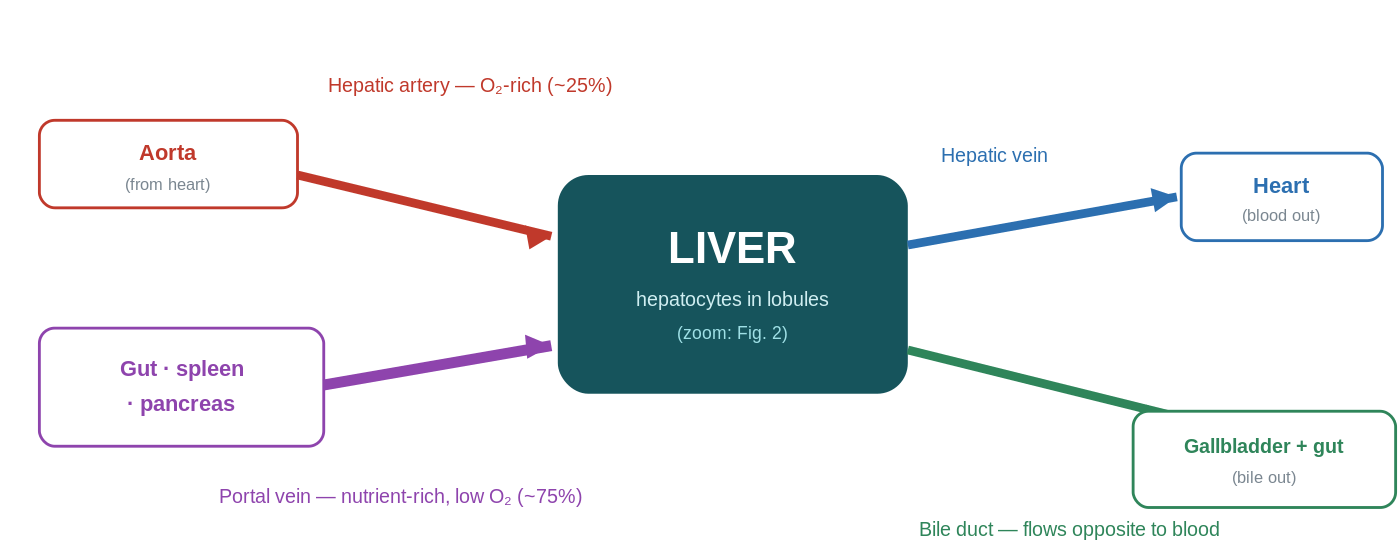
\includegraphics[width=0.85\linewidth]{fig1.png}
\caption{The liver in its plumbing. Two supplies enter together at the portal triads --- the
\textbf{portal vein} (from gut, spleen, pancreas; nutrient-rich, low O$_2$) and the \textbf{hepatic
artery} (O$_2$-rich, from the aorta) --- mix through the sinusoids and leave as blood via the
\textbf{hepatic vein} to the heart. \textbf{Bile} exits the other way, through the bile ducts to the
gallbladder and gut. Figure~\ref{fig:lobule} zooms into one lobule.}
\label{fig:plumbing}
\end{figure}

\subsection{The lobule, the gradient, and zonation}
\label{sec:lobule}

The liver's repeating unit is the \textbf{lobule}, a roughly hexagonal tile about 0.5--1\,mm across.
Blood enters at the corners through the \textbf{portal triads} and flows inward to a \textbf{central
vein} at the centre. Along that journey --- the \textbf{porto--central axis} --- the blood gives up its
oxygen and nutrients, so a cell's chemical environment depends entirely on how far along the axis it
sits: relatively oxygen-rich at the portal edge, oxygen-poor at the centre.

\begin{figure}[h]
\centering
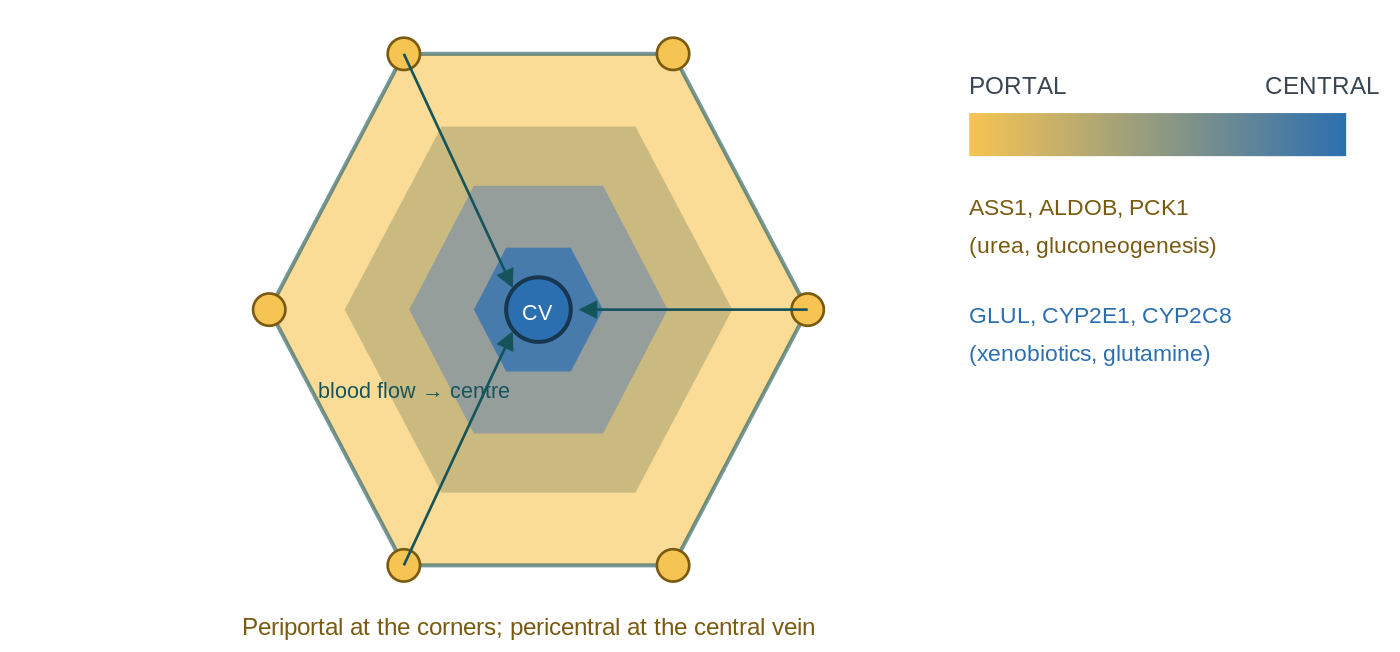
\includegraphics[width=0.8\linewidth]{fig2.png}
\caption{The lobule. Blood flows inward from the oxygen-rich portal corners to the oxygen-poor central
vein; zonation runs along that path. The bands are \emph{schematic}: real zonation is a smooth gradient
along the sinusoids (acinus zones~1--3), not discrete rings, and bile drains the opposite way (toward
the portal triads). Representative marker genes for each end are shown.}
\label{fig:lobule}
\end{figure}

Because the environment changes smoothly along the axis, hepatocytes specialise smoothly too. This
division of labour is called \textbf{liver zonation}. Broadly, the \textbf{periportal} end runs much
of the urea cycle (\gene{ASS1}) and gluconeogenesis (\gene{PCK1}, \gene{ALDOB}), while the
\textbf{pericentral} end runs glutamine synthesis (\gene{GLUL}) and cytochrome-P450 xenobiotic
metabolism (\gene{CYP2E1}, \gene{CYP2C8}).

\aside{A human-specific result, and why we read markers from the data}{A key finding of Paper~2 is
that several functions long assumed periportal are actually \textbf{pericentrally shifted in humans}
--- the gluconeogenic gene \gene{PCK2} and the urea-cycle enzymes \gene{ASL}/\gene{OTC}/\gene{NAGS}
among them, while \gene{ASS1} stays periportal. So we take marker sets \emph{empirically from the
data}, not from the mouse textbook.}

Crucially the cell carries out this specialisation by \emph{switching genes on and off} in proportion
to its position. So a hepatocyte's set of active genes is, in effect, a readout of where it sits.
\textbf{That is the hinge of the whole project:} if position is encoded in expression, then position
can be decoded back out of expression --- even after the physical location is gone.

\subsection{The disease that degrades it: the MASLD spectrum}
\label{sec:masld}

Both papers study \textbf{MASLD} (metabolic dysfunction-associated steatotic liver disease, formerly
NAFLD), the commonest chronic liver disease, which advances through ordered stages
(Table~\ref{tab:stages}).

\begin{table}[h]
\centering\small
\caption{The MASLD disease spectrum --- an \emph{ordered} axis (this ordering is what H1 exploits).}
\label{tab:stages}
\begin{tabular}{@{}lll@{}}
\toprule
\textbf{Stage} & \textbf{What happens} & \textbf{Hallmark}\\
\midrule
Healthy & Normal architecture and zonation & baseline\\
MASLD / steatosis & Fat droplets accumulate inside hepatocytes & steatosis\\
MASH & Fat $+$ inflammation $+$ hepatocyte injury (ballooning) & inflammation\\
Cirrhosis & Scarring (fibrosis) replaces working tissue & fibrosis\\
End-stage & Architecture destroyed; regenerative nodules & organ failure\\
\bottomrule
\end{tabular}
\end{table}

\textbf{Terminology.} MASLD/MASH is the current name; the Paper~1 dataset and older literature label
the same stages \textbf{NAFLD/NASH}. We use MASLD/MASH in prose but keep the dataset's own labels when
reading its metadata.

\textbf{Why it happens (in brief).} MASLD is a disease of metabolic overload. Chronic excess calories
and \textbf{insulin resistance} push more fatty acids into hepatocytes than they can burn or export,
so triglyceride accumulates as droplets (\textbf{steatosis}). When the lipid load outstrips the cell's
capacity it turns toxic (\emph{lipotoxicity}): mitochondrial and ER stress, reactive-oxygen damage,
hepatocyte injury and death. That damage recruits immune cells (inflammation $=$ \textbf{MASH}) and
activates hepatic stellate cells to lay down collagen scar (\textbf{fibrosis $\to$ cirrhosis}).
Genetics (e.g.\ \gene{PNPLA3}, \gene{TM6SF2}) and the gut--metabolic milieu tune individual risk.

\aside{Is de-zonation a mechanism or a symptom?}{Mostly a \textbf{readout}: zonation is maintained by
spatial signalling gradients (notably Wnt/$\beta$-catenin and oxygen), and metabolic stress plus
disrupted Wnt degrade it --- so de-zonation largely \emph{reports} how far cellular identity has
unravelled rather than causing the disease. But it is not cosmetic: the two ends run \emph{different}
jobs, so losing the gradient means specific liver functions fail in a specific order. That is why we
map it: a quantitative severity marker finer than histology, a pointer to which functions degrade
first, a possible early pre-fibrotic flag, and a link to the plasticity route tied to cancer risk.}

\subsection{The two ways identity breaks --- and why keeping them apart is the whole point}
\label{sec:twobreaks}

As disease advances, the orderly lobule degrades in two \emph{distinct} ways. \textbf{De-zonation} is
loss of normal \emph{zonal restriction} within the hepatocyte population: genes that should be confined
to one end of the porto--central axis become blurred, silenced, or co-expressed with the opposite
program. (Co-expression of opposite ends is one important mode; global loss of a program and flattening
of the gradient are others --- \S\ref{sec:popprop} tells them apart.) \textbf{Epithelial plasticity}
is loss of identity \emph{across} cell types: the boundary between hepatocyte and cholangiocyte
identity blurs, producing \textbf{biphenotypic} cells expressing markers of \emph{both} lineages. This
is molecular, not physical --- no cell crawls into a duct; the gene-expression programs mix. (Paper~1
reports such transdifferentiation with organoid $+$ PI3K--AKT--mTOR evidence; the in-vivo
directionality is complex, so we treat it as boundary-blurring, not a clean one-way switch.)

So the contrast is clean: de-zonation $=$ a hepatocyte forgetting \emph{where on the axis} it belongs;
plasticity $=$ a hepatocyte forgetting \emph{that it is a hepatocyte at all}.

\begin{table}[h]
\centering\small
\caption{De-zonation vs plasticity --- they sound identical but cross \emph{different} boundaries.
H3 asks whether they are the same cells.}
\label{tab:dezvsplast}
\begin{tabular}{@{}p{0.22\linewidth} p{0.36\linewidth} p{0.36\linewidth}@{}}
\toprule
 & \textbf{De-zonation} & \textbf{Plasticity}\\
\midrule
Boundary crossed & \emph{Position} within the hepatocyte (portal vs central end) & \emph{Cell type}
identity (hepatocyte vs cholangiocyte)\\
Co-expressed pair & pericentral $+$ periportal (e.g.\ \gene{CYP2E1} $+$ \gene{ASS1}) in one cell &
hepatocyte $+$ bile-duct (e.g.\ \gene{ALB} $+$ \gene{KRT7}) in one cell\\
Still a hepatocyte? & Yes --- it just lost its \emph{address} on the assembly line & Drifting --- it
is forgetting its \emph{profession} altogether\\
\bottomrule
\end{tabular}
\end{table}

\textbf{Analogy.} A factory worker who forgets \emph{which station} they man (de-zonation) is still a
factory worker; one who forgets they \emph{work in this factory at all} (plasticity) is something else.
De-zonation is the milder, earlier slip; plasticity the deeper one. \textbf{H3 tests whether losing
your address predicts losing your job.}

\aside{The need this sets up}{To measure de-zonation we would need two things we do not obviously
possess together: (1)~a trustworthy, quantitative map of \textbf{healthy} zonation (a ruler), and
(2)~a large population of \textbf{diseased} cells, spanning every stage, to lay against that ruler.
The next section shows that exactly these two things exist --- in two separate papers --- and that
nobody has put them together.}

\clearpage
% ====================================================================
\section{The data \& the gap}
% ====================================================================

Our need has two halves --- a healthy ruler and diseased cells --- and there happen to be two papers,
each supplying exactly one half. To see why they fit together (and why neither alone is enough), we
first need one idea about \emph{how} the measurements are made.

\subsection{Two ways to measure a tissue: keep the map, or dissolve it}

In ordinary sequencing, a molecule's physical position on the instrument is meaningless --- genomic
identity comes only from alignment. The whole idea of spatial transcriptomics is to make a position
mean something biological again: not on the flow cell, but in the tissue. There are two families of
technique, and the difference between them \emph{is} our opportunity.

\begin{itemize}[leftmargin=1.4em]
\item \textbf{Single-nucleus RNA-seq (snRNA-seq)} \emph{dissolves the tissue first.} Lyse the cells and
release nuclei into a suspension; pool and shuffle them; capture each in its own droplet with a
barcoded bead carrying a \textbf{cell barcode}; tag every captured mRNA with a \textbf{UMI} (unique
molecular identifier) so PCR duplicates collapse; reverse-transcribe, amplify, sequence, and end with a
nuclei\,$\times$\,genes count matrix. The reward is enormous --- you read essentially the whole
transcriptome of each cell, and nuclei survive the freezing and fibrosis that would destroy whole
cells, which is the only reason late-stage scarred tissue can be profiled at all. The price is
irreversible: the moment nuclei go into suspension, \textbf{which lobule or axis-position each came from
is gone forever.} (scRNA-seq is the whole-cell cousin; both are dissociated methods.)
\item \textbf{Spatial transcriptomics} measures expression \emph{without} dissociating --- on an
intact tissue section, so each measurement carries its $(x,y)$ coordinate. The workhorse, \textbf{10x
Visium}, lays the slice on a slide printed with a grid of barcoded \textbf{spots} ($\sim$55\,$\mu$m, a
few cells each); every transcript inherits its spot's barcode, so position is retained. Higher-resolution
variants --- \textbf{Visium HD} (a fine 2--8\,$\mu$m grid), \textbf{MERFISH} (imaging that counts a few
hundred chosen genes molecule-by-molecule), and \textbf{PhenoCycler/CODEX} (cyclic antibody imaging of
proteins) --- trade transcriptome breadth for resolution.
\end{itemize}

No method gives everything: spatial methods sit on a triangle of competing goods --- transcriptome
breadth, spatial resolution, and sensitivity --- and you choose your corner to match the question. The
headline trade is simple: dissociated $=$ all genes, no position; spatial $=$ position kept, with some
cost in breadth or sensitivity.

\aside{Two different ``losses'' --- keep them separate, they matter all the way through}{(1)~\textbf{
Technical} loss of coordinates: snRNA-seq dissolves the tissue, so we no longer know where a cell sat.
This is a limitation of the \emph{instrument}. (2)~\textbf{Biological} de-zonation: in disease the cell
itself loses its zonal identity. This is the \emph{phenomenon we study}. The whole project is: use a
spatial reference to undo loss~(1) just well enough to measure loss~(2).}

\aside{The move at the heart of the project: spatial as a ruler}{A spatial dataset is a reference map
in which expression is tied to position --- for the liver, where each profile sits along the
porto--central axis. We \textbf{learn} from that reference the relationship ``this expression pattern
$\to$ this zone-index.'' Then we take the dissociated disease data, which on its own has no coordinates,
and \textbf{apply} that learned mapping to decode an inferred position per cell. The spatial map is the
ruler; the dissociated data are the measurements we re-place onto it. The reference effectively donates
its coordinate system to data that has none --- which lets us ask spatial questions on a dataset with
no spatial information of its own.}

\subsection{Paper~2 --- the healthy ruler}

\noindent\textit{Yakubovsky, Bahar Halpern, Shir et~al.\ (Itzkovitz lab). A spatial atlas of the
healthy human liver from live donors. Nature (2026). doi:10.1038/s41586-026-10377-y.}

This paper supplies our ruler. Its key move was to obtain genuinely healthy human liver from
\textbf{living} donors (ordinary ``normal'' references come from brain-dead organ donors, whose livers
are metabolically disturbed), and to profile 16 samples with the full spatial battery plus snRNA-seq.
From the spatial data it reconstructed a quantitative porto--central \textbf{zone index} per spot and
identified the genes that vary most cleanly along the axis.

\aside{What to extract from Paper~2}{\textbf{Figure~2 is the one that matters} --- the zonation
reconstruction. The paper analyses \textbf{1{,}724 hepatocyte-specific genes}, of which \textbf{1{,}141
show significant zonal differences} ($q<0.25$), each with a gene-zonation score, and normalizes
expression as z-scores of $\log_{10}$ UMI-sum-normalized values --- match that normalization so the
signatures transfer. Pull: (i)~the ranked zonated-gene table $\to$ the transcriptome-wide
pericentral/periportal signatures; (ii)~the landmark genes anchoring each end (pericentral
\gene{CYP2E1}, \gene{CYP2C8}, \gene{GLUL}, and the human-specific \gene{PCK2}; periportal \gene{ASS1},
\gene{ALDOB}, \gene{PCK1}) $\to$ the faithful landmark baseline; (iii)~the snRNA-seq data and the
script assigning zonation to those nuclei (the classifier training set, \S\ref{sec:workplan}).}

\subsection{Paper~1 --- the diseased cells}

\noindent\textit{Gribben, Galanakis, Calderwood et~al.\ (Vallier, Mohorianu, Allison labs).
Acquisition of epithelial plasticity in human chronic liver disease. Nature (2024).
doi:10.1038/s41586-024-07465-2.}

This paper supplies the cells to test. It profiled \textbf{47 liver biopsies} by snRNA-seq across the
entire spectrum --- healthy ($n=4$), MASLD/NAFLD ($n=7$), MASH ($n=27$), cirrhosis ($n=4$), end-stage
($n=5$) --- yielding $\sim$100{,}000 QC-passing nuclei including \textbf{69{,}426 hepatocytes}. Its
headline biology is transdifferentiation between hepatocytes and cholangiocytes, driven by
PI3K--AKT--mTOR; for us, the relevant secondary observation is that hepatocytes lose zonation --- but
it reports this only qualitatively.

\aside{What to extract from Paper~1}{\textbf{Figure~1c--e} defines the experiment and the cell-type
annotation (nuclei isolated by tissue lysis and FACS from snap-frozen biopsies; 10x; CellRanger
v5.0.0), the annotated UMAP, and the marker bubble-plot used to confirm hepatocytes (\gene{ALB}).
\textbf{Figure~2} is their zonation evidence --- a hepatocyte UMAP split by stage, and a correlation of
pericentral vs periportal marker expression across progression --- precisely the qualitative result we
turn quantitative and continuous. Extract: (i)~the cell-type and stage fields from metadata;
(ii)~their pericentral (\gene{GLUL}, \gene{AXIN2}) and periportal (\gene{ASS1}, \gene{HAL}) markers;
(iii)~the plasticity markers for H3 (\gene{KRT7}, \gene{KRT19}, \gene{SOX9}, plus \gene{SOX4},
\gene{KRT23}, \gene{NCAM1}). One caveat: GEO samples GSM6112262 and GSM6112263 had swapped metadata
(fixed June 2025) --- use the corrected version.}

\subsection{The gap --- mirror images neither paper has joined}

\begin{table}[h]
\centering\small
\caption{The two datasets are complementary halves of one puzzle.}
\label{tab:gap}
\begin{tabular}{@{}lll@{}}
\toprule
 & \textbf{Paper~2 (the ruler)} & \textbf{Paper~1 (the cells)}\\
\midrule
Spatial coordinates & Kept (Visium, MERFISH) & Destroyed (snRNA-seq)\\
Disease coverage & Healthy $+$ early steatosis only & Full spectrum, healthy $\to$ end-stage\\
Zonation & Quantitative, per-spot ruler & Noted only qualitatively\\
Scale & 44{,}243 spots ($+$ snRNA-seq) & 69{,}426 hepatocytes\\
\bottomrule
\end{tabular}
\end{table}

\begin{figure}[h]
\centering
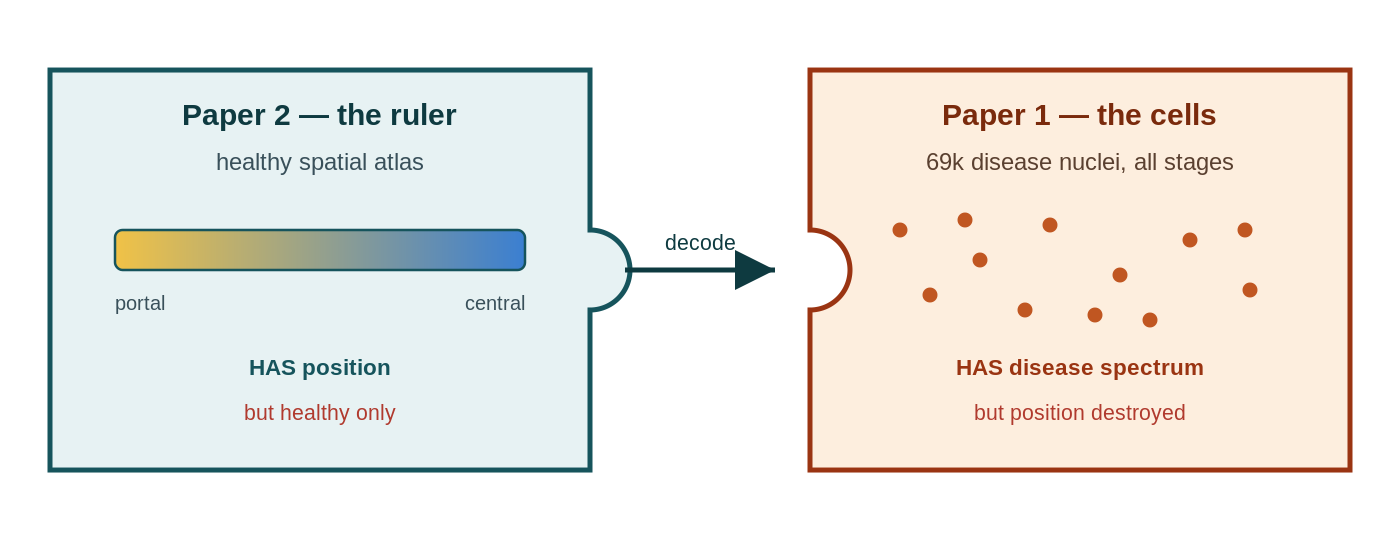
\includegraphics[width=0.8\linewidth]{fig3.png}
\caption{Two halves of one puzzle. The healthy atlas (left) carries a quantitative portal$\to$central
position but no disease; the single-nucleus cohort (right) spans the whole disease course but has thrown
its positions away. The project's one move is to fit the left piece's ruler into the right piece's cells
--- using the healthy gradient to assign each diseased nucleus a pseudo-zonation coordinate.}
\label{fig:jigsaw}
\end{figure}

One paper has the \textbf{map} but no disease; the other has the \textbf{disease} but no map. Both are
recent --- Paper~1 (2024), Paper~2 (2026) --- and each was built to answer its own question, so no one
has yet used the healthy spatial ruler to decode the disease cohort. That untaken step is our project.

\aside{``But Paper~1 already showed zonation loss''}{Paper~1's zonation evidence is a UMAP, a
correlation of \emph{two} marker genes, and microscopy of a handful of marker proteins in healthy vs
end-stage tissue. That is \textbf{qualitative} (you look and see it's messier), \textbf{discrete} (two
extremes), and \textbf{narrow} (a few markers). We add three things it lacks: (1)~\textbf{quantitative}
--- a de-zonation \emph{number} per stage with confidence intervals and a significance test;
(2)~\textbf{continuous} --- every one of the 69{,}426 hepatocytes gets a real-valued position, tracked
across all five stages as a curve, not two snapshots; (3)~\textbf{transcriptome-wide} --- position read
from the whole zonation program (the $\sim$1{,}141 significantly zonated genes among 1{,}724
hepatocyte-specific genes) via an external healthy reference, not 2--3 markers by eye. In one line: they
showed \emph{that} zonation is lost; we measure \emph{how much, where on the axis, and with what
significance}, across the entire disease course.}

\clearpage
% ====================================================================
\section{Research question \& hypotheses}
% ====================================================================

\aside{Research question}{Using the healthy porto--central zonation ruler from Paper~2, can we assign a
quantitative pseudo-zonation coordinate to every spatially-blind hepatocyte in Paper~1, and so measure
\textbf{how, and how much, hepatocyte zonation degrades as MASLD advances from healthy to end-stage}
--- and is that degradation linked to the transdifferentiation Paper~1 reported?}

Each hypothesis below is what we hope to show (the \emph{alternative}); every statistical test silently
compares it against its \textbf{null}, the boring ``no-effect'' world, and a p-value measures evidence
against that null. The full statistical toolkit is in \S\ref{sec:stats}; the tests are named here.

\begin{table}[h]
\centering\small
\caption{The three hypotheses, their nulls, and the test for each.}
\label{tab:hyp}
\begin{tabular}{@{}p{0.34\linewidth} p{0.30\linewidth} p{0.30\linewidth}@{}}
\toprule
\textbf{Hypothesis (alternative)} & \textbf{Null ($H_0$)} & \textbf{Test}\\
\midrule
\textbf{H1 --- monotonic erosion.} A de-zonation score rises
Healthy$\to$MASLD$\to$MASH$\to$cirrhosis$\to$end-stage. & The score is flat across stages --- no
association with disease. & Ordered trend (Jonckheere--Terpstra / Spearman on stage rank)\\
\textbf{H2 --- zone-specific vulnerability.} Particular programs (e.g.\ pericentral CYP detox) collapse
earlier/faster. & A gene's zonal pattern does not change across stages. & Pseudobulk DE $+$ BH-FDR\\
\textbf{H3 --- plasticity link.} The most de-zonated hepatocytes are the ones gaining cholangiocyte
identity. & De-zonation and plasticity scores are independent. & Within-donor correlation /
Mann--Whitney\\
\bottomrule
\end{tabular}
\end{table}

\subsection{H1 --- does zonation erode as disease advances?}

\textbf{Claim:} a single de-zonation score climbs steadily Healthy$\to$NAFLD$\to$NASH$\to$cirrhosis
$\to$end-stage. The score is a \emph{population} metric --- e.g.\ the weakening of
pericentral--periportal mutual exclusivity, or the narrowing of the coordinate's spread --- \textbf{not}
any single cell's position (\S\ref{sec:popprop}). \textbf{Null:} the score is flat --- unrelated to
stage.

\textbf{The test, plainly.} Our stages have a natural order, so we ask whether the score moves
\emph{monotonically} along it. \textbf{Spearman correlation} ($\rho$) measures whether two things rise
or fall together by rank ($\rho=+1$ perfectly increasing, 0 no relationship). The
\textbf{Jonckheere--Terpstra} test is the dedicated significance test for an \emph{ordered} trend
across ordered groups. \textbf{Pass:} a significant trend ($\rho>0$, $p<0.05$) that survives
donor-level resampling. \textbf{If it fails (still useful):} a flat score means zonation is surprisingly
robust; a rise-then-plateau means the damage saturates early.

\begin{figure}[h]
\centering
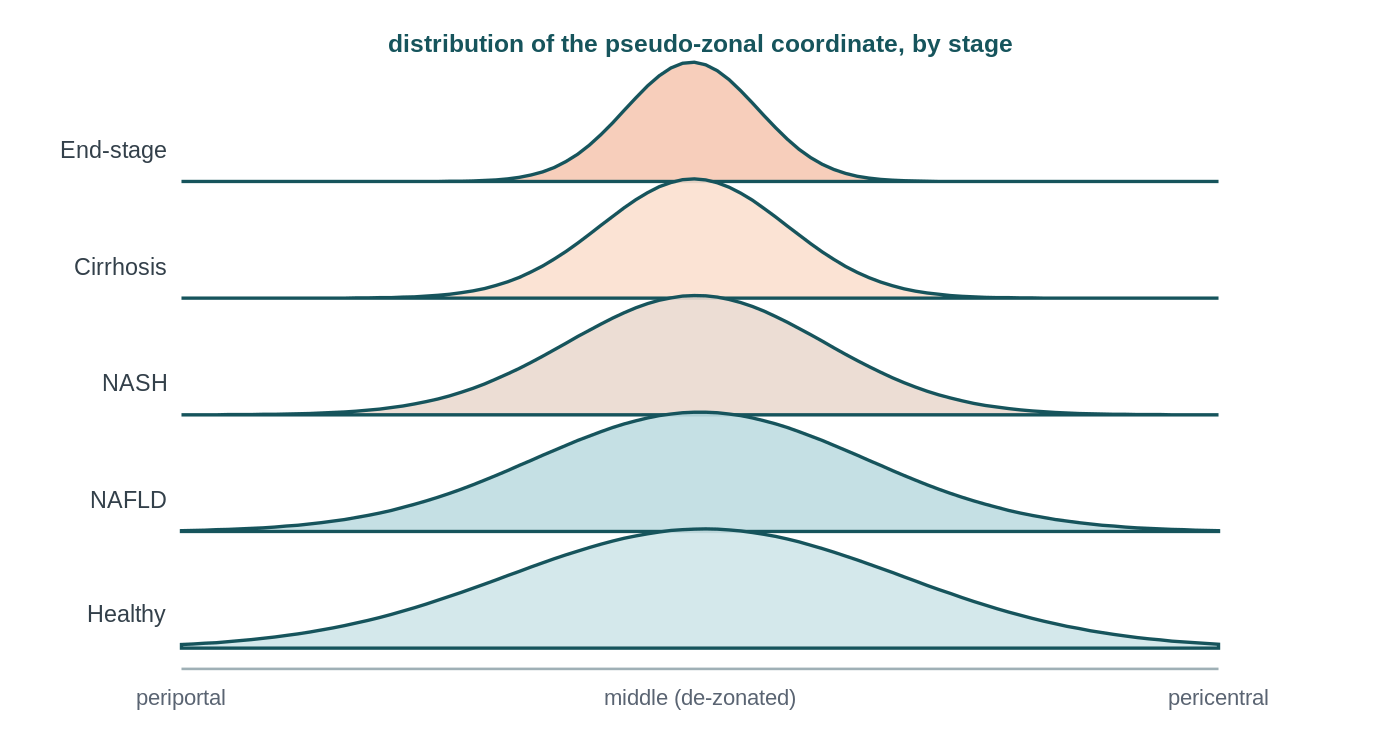
\includegraphics[width=0.8\linewidth]{fig4.png}
\caption{What H1 should look like (illustrative). Zonation is a \textbf{continuum}, so the healthy
coordinate is a \emph{single wide hump} (cells occupy every position along the axis) --- \emph{not} two
peaks. The signal of healthy zonation is the \textbf{width} (and that markers track the axis,
Fig.~\ref{fig:scatter}), not bumpiness. As disease advances the hump \textbf{narrows} toward the middle:
cells stop committing to either end. H1 measures that narrowing (coordinate spread/variance) plus the
weakening pericentral--periportal anti-correlation --- one number per donor, tested across stages.}
\label{fig:ridgeline}
\end{figure}

\subsection{H2 --- which gene programs collapse, and where on the axis?}

\textbf{Claim:} the collapse is not uniform --- specific programs (e.g.\ pericentral CYP detox genes)
lose their zonal pattern earlier/faster. \textbf{Null:} a given gene's zonal pattern does not change
across stages. \textbf{The test, plainly.} We bin cells into pseudo-zones (portal / mid / central) and,
within a zone, test each gene for change across stages --- \textbf{differential expression}, run at the
donor level by pseudobulk (\S\ref{sec:stats}). Testing $\sim$20{,}000 genes at $p<0.05$ would give
$\sim$1{,}000 false hits from noise alone, so we apply \textbf{Benjamini--Hochberg FDR}.
\textbf{Pass:} a coherent set of genes at $q<0.05$ whose loss explains the collapse, ideally enriched
for known zonated programs. \textbf{If it fails (still useful):} no significant genes means the collapse
is diffuse rather than program-specific --- itself a statement about \emph{how} zonation breaks.

\subsection{H3 --- do the de-zonated cells become the plastic ones?}

\textbf{Claim:} the hepatocytes that have lost zonal identity are the same ones drifting toward
cholangiocyte identity (gaining \gene{KRT7}/\gene{KRT19}). \textbf{Null:} de-zonation and plasticity
are independent. \textbf{The test, plainly.} We score each hepatocyte for a plasticity signature, split
cells into ``de-zonated'' vs ``still-zonated,'' and ask whether the de-zonated group has higher
plasticity (\textbf{Mann--Whitney U}). Crucially we test this \emph{within stage / within donor} ---
\emph{not} pooled across all cells, where late disease simply having more of both would fake a link (the
stage confound, \S\ref{sec:stats}). \textbf{Pass:} de-zonated hepatocytes show significantly higher
plasticity ($p<0.05$) and the two scores correlate positively within donors. \textbf{If it fails (still
useful):} independence would mean losing zonal identity and gaining duct identity are separate processes.

\aside{Why this is not reproduction}{Neither paper computed a cross-dataset zonation coordinate for the
disease cohort, a stage-resolved collapse curve, or the de-zonation\,$\leftrightarrow$\,plasticity link.
We use Paper~2 strictly as a \emph{decoder} for Paper~1. The lasting value is threefold and none is made
redundant by a future real-spatial study: a reusable reference-based decoder for the many dissociated
atlases with no spatial data; a mechanistic ordering of which zonal programs lose legibility first (H2);
and a principled failure analysis of when and how the healthy program stops being legible
(\S\ref{sec:rulervalid}), tied to plasticity (H3).}

\clearpage
% ====================================================================
\section{Methods: from data to a position-number}
% ====================================================================

\noindent\emph{Section~\ref{sec:lobule} promised that position is written into expression. This section
turns that promise into a procedure, building it one forced step at a time: each tool appears only
because the previous step created a problem that demands it. Nothing here is a tool for its own sake.}

\subsection{Where we begin: the count table}

After sequencing, the data is one giant table: a row per gene, a column per cell, each entry the number
of molecules (\textbf{UMIs}) of that gene caught in that cell. Tens of thousands of each; everything
downstream is arithmetic on this table. Reaching it is the alignment of Exercise~1 (placing reads on
the genome) and the molecule-counting of Exercise~2 (deduplicating PCR copies into unique counts) ---
but the published datasets hand us the finished table, so that is our starting line.

\subsection{The table lies --- so first we clean it (QC \& normalization)}

Two flaws make the raw table unsafe. \textbf{First, not every column is a real cell.} Empty droplets,
debris, and dying or leaky nuclei produce junk columns; if kept they later masquerade as ``confused''
cells and fake the very signal we hunt. So we discard them --- filtering on too-few molecules, too-few
detected genes, or too-high mitochondrial content (a dying-cell tell). This is \textbf{quality control
(QC)}. \textbf{Second, the surviving numbers aren't comparable:} a cell sequenced twice as deeply shows
twice the counts for a purely technical reason. So we rescale every cell to a common depth, then take a
logarithm --- so a \emph{doubling} counts the same whether a gene goes $100\to200$ or $1000\to2000$,
the multiplicative scale biology actually lives on (we use $\log(1+x)$, because $\log 0$ is undefined
and the table is full of zeros). This is \textbf{normalization}.

Concretely, our normalization is counts-per-10k $\to$ $\log$1p $\to$ per-gene z-score. Writing
$c_{gi}$ for the raw count of gene $g$ in cell $i$ and $N_i=\sum_g c_{gi}$ for that cell's total:
\begin{align}
\text{CP10k:}\quad & \tilde c_{gi} = \frac{c_{gi}}{N_i}\times 10^4, \\
\text{log1p:}\quad & x_{gi} = \log\!\big(1+\tilde c_{gi}\big), \\
\text{z-score:}\quad & z_{gi} = \frac{x_{gi}-\mu_g}{\sigma_g},
\qquad \mu_g=\operatorname{mean}_i x_{gi},\ \ \sigma_g=\operatorname{sd}_i x_{gi}.
\end{align}
The z-score puts every gene on a common, unit-variance scale so that pooling many genes into one score
is not dominated by a few highly-expressed ones, and so the units match Paper~2's
($z$ of $\log$ UMI-sum-normalized) and the signatures transfer.

\aside{QC we inherit; normalization we redo --- exactly why}{Paper~1's authors already cell-filtered
their published object, so we \textbf{inherit their QC} (plus a one-line check that the kept cells are
\gene{ALB}-expressing hepatocytes); we do \emph{not} re-filter from scratch. But we \textbf{re-normalize
from the raw counts}, for three reasons. \textbf{(1)~A cross-dataset transfer needs identical
preprocessing} --- we score Paper~1 against Paper~2-derived signatures and apply a Paper~2-trained
classifier, so both sides must traverse the \emph{same} pipeline, starting from counts.
\textbf{(2)~Their processed matrix is gene-incomplete} --- a Seurat object carries multiple slots: the
raw \code{counts} slot holds \emph{every} gene ($\sim$30k), while the \code{scale.data} slot usually
holds only the $\sim$2{,}000 highly-variable genes (covariates regressed out), so several signature
genes may be absent or differently scaled there. We pull \code{counts}, not \code{scale.data}.
\textbf{(3)~Reproducibility} --- a transparent pipeline we control can be defended in the report,
instead of an undocumented, software-version-specific one.}

\subsection{The zeros are a trap --- and the trap dictates the method}

Most of the table is zeros, and a zero is ambiguous: the gene may be genuinely off, or
on-but-\emph{missed}. Only a fraction of a cell's molecules are ever captured, so a gene present in a
few copies frequently reads zero by pure chance --- the same Poisson sampling you met modelling library
complexity in Exercise~2 (the probability of seeing none is $e^{-\lambda}$, large when the expected
count $\lambda$ is small). The missed-but-present zero is called \textbf{dropout}, and snRNA-seq is
especially prone to it because a nucleus holds little RNA. The conclusion is decisive and shapes
everything after it: \textbf{no single gene's value in a single cell can be trusted.}

\subsection{Therefore: read position from many genes at once (signature scoring)}
\label{sec:scoring}

Because one gene is unreliable but the zonation \emph{program} spans many genes (Paper~2 finds
$\sim$1{,}141 significantly zonated hepatocyte genes, \S3.2), we read position from \emph{many} genes
pooled together --- which also averages out the random per-cell dropout. A \textbf{signature score} is
the (normalized, scaled, background-subtracted) \emph{mean} expression of a chosen gene set.
``Background-subtracted'' means: from each cell's mean over the signature genes we subtract that same
cell's mean over a matched set of random \emph{control} genes, so the score reflects the signature
\emph{specifically} rather than how highly-expressing / deeply-sequenced the cell is overall (exactly
what Scanpy's \code{score\_genes} does). Writing $S$ for a signature gene set and $B$ for a matched
background set, the score of cell $i$ is
\begin{equation}
\text{score}_i(S) \;=\; \frac{1}{|S|}\sum_{g\in S} z_{gi}\;-\;\frac{1}{|B|}\sum_{g\in B} z_{gi}.
\end{equation}
We build a \textbf{pericentral} and a \textbf{periportal} signature from Paper~2's ruler and define a
single coordinate per cell:
\begin{equation}
\boxed{\ \text{zonation\_coord}_i \;=\; \text{score}_i(\mathrm{PERICENTRAL}) \;-\;
\text{score}_i(\mathrm{PERIPORTAL}).\ }
\end{equation}
High $=$ pericentral-like, low $=$ periportal-like; a middle value is \emph{ambiguous} --- it can mean
``expresses neither'' \emph{or} ``expresses both,'' so a single cell's middling coordinate is only a
\emph{candidate} for de-zonation, confirmed by the population-level structural metrics below, not by the
coordinate alone. The coordinate is a \emph{signed real number} (sign $=$ which end; magnitude $=$ how
strongly committed), centred near zero --- \textbf{not} a 0--1 probability; probabilities come later,
from the classifier (\S\ref{sec:classifier}).

\aside{The signature, run both ways --- landmark \emph{and} transcriptome-wide}{We compute the
coordinate with \textbf{two} gene schemes and report both, checking they agree.
\textbf{(a)~The exact Paper~2 landmark set} --- the verbatim 20$+$20 pericentral/periportal landmark
genes Paper~2 used to seed its axis. This is \emph{faithful to the original landmark/marker-based plan}
and is the interpretable sanity baseline.
\textbf{(b)~The full transcriptome-wide program} --- the $\sim$1{,}640 significantly-zonated hepatocyte
genes ($q<0.05$, well-expressed, present in Paper~1; PC/PP $=$ 1{,}273\,/\,364). This is the
\textbf{default}, and a deliberate strengthening: it reads position from the \emph{entire} program
rather than a handful of markers by eye, which is the whole motivation of the project and is also what
makes the non-circular held-out-gene test (\S\ref{sec:workplan}, Step~7) meaningful. Two further sets
bridge them as robustness checks --- a $\sim$100-gene \code{expanded} set (landmark $\cup$ core $\cup$
top-ranked) and a curated 13/8-gene \code{core}. \textbf{Honest framing:} transcriptome-wide is the
headline because it is stronger, but we run the landmark set alongside and show the collapse is the
\emph{same} either way --- so the result is not an artefact of choosing a large gene set. (An earlier
draft mistakenly made the 20-gene landmark set the default, silently contradicting the
transcriptome-wide motivation; corrected here.)}

\noindent\textbf{In code.} \code{src/steps/step4\_score.py} --- \code{coord = mean\_z(pericentral) -
mean\_z(periportal)}; default gene sets are \code{signatures/*\_full.txt} (via
\code{config.DEFAULT\_SET="full"}); switch with \code{config.signature\_files("paper2\_landmark")} etc.
PCA, UMAP and clustering are used only as scaffolding here (to isolate hepatocytes and draw a
score-coloured map), because Paper~1 already provides cell-type labels --- the result comes from the
coordinate, not the picture.

\begin{figure}[h]
\centering
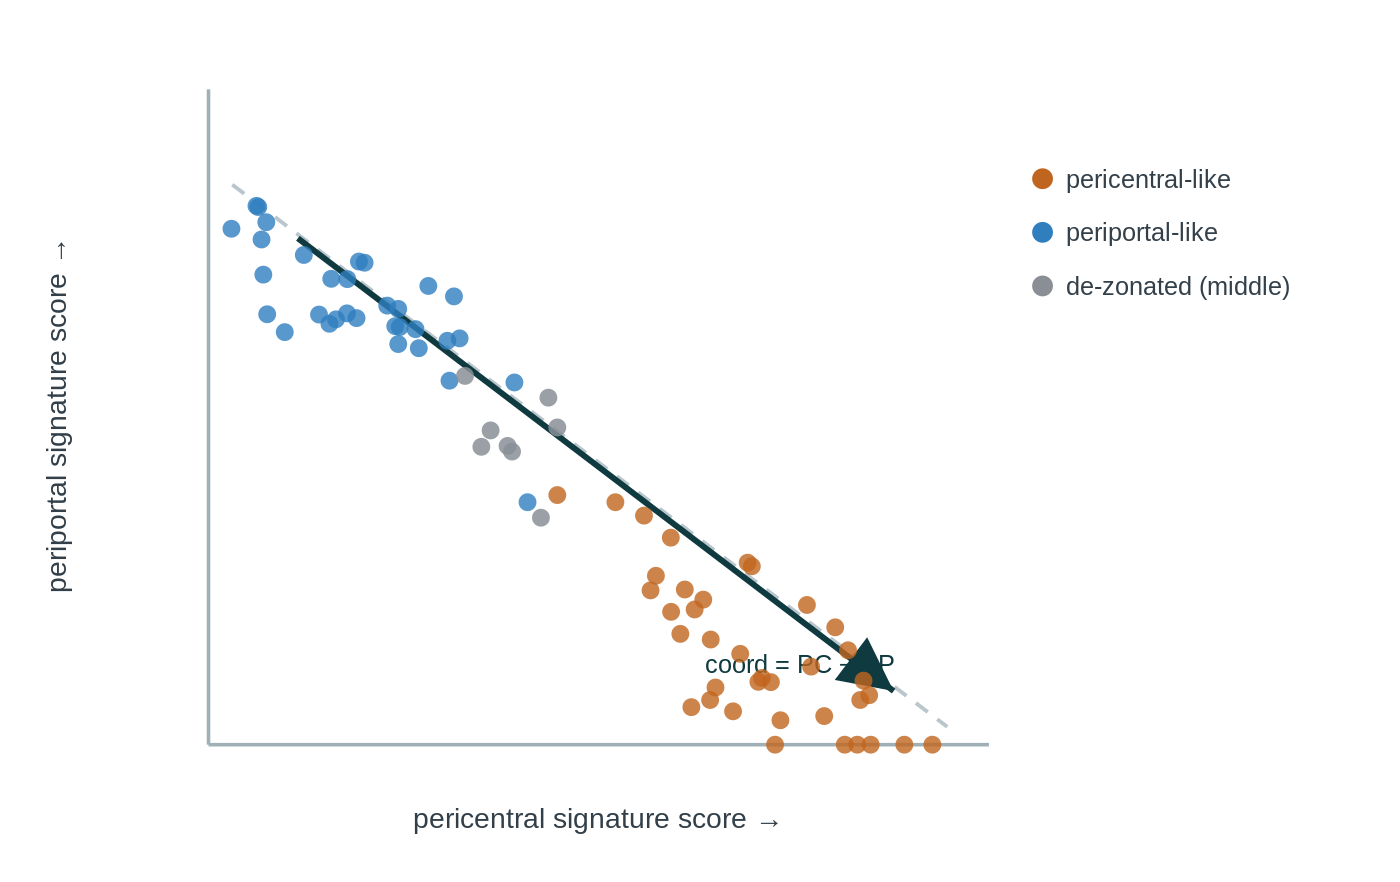
\includegraphics[width=0.75\linewidth]{fig5.png}
\caption{How one coordinate is read from two scores. Each dot is a cell, placed by its pericentral
score ($x$) and periportal score ($y$). In healthy tissue the two are \textbf{mutually exclusive} ---
cells fall into two anticorrelated clouds --- and a single number, $\text{coord}=\text{PC}-\text{PP}$,
captures where each sits on the portal$\leftrightarrow$central axis. The grey ``de-zonated'' cells in
the middle --- high on neither or muddled on both --- are exactly what proliferates as disease erases
the separation (Fig.~\ref{fig:ridgeline}). Computing the coordinate with both the landmark and the
transcriptome-wide sets and showing they agree is itself evidence the signal is robust.}
\label{fig:scatter}
\end{figure}

\aside{Honesty guardrail}{The ruler is a \textbf{1D} axis, so we recover a \textbf{pseudo-zonation
coordinate}, never a physical $(x,y)$ location. We say ``reconstructed zonation coordinate,'' not
``predicted spatial position.''}

\subsection{A stronger reader: a zone classifier, and why its confusion is the signal}
\label{sec:classifier}

The signature score is robust but blunt --- it gives one number and no sense of how \emph{sure} we are.
A classifier adds exactly that. We show a model many hepatocytes whose zone is already \emph{known}
(``training''), and it learns the mapping from a cell's expression to its zone. Then, for a new cell, it
outputs not a single label but a \textbf{probability for each zone} --- e.g.\ [central~0.92, mid~0.06,
portal~0.02].

\textbf{Why the probabilities are the whole point.} The \emph{shape} of that probability vector
measures confidence, and lost confidence \emph{is} de-zonation. A healthy, clearly-zonated cell gives a
\textbf{peaked} vector (the model is sure). A de-zonated cell --- now part-pericentral, part-periportal
--- gives a \textbf{flat} vector (e.g.\ 0.40/0.35/0.25): the model genuinely can't tell, because the
cell no longer commits to a zone. We compress ``peaked vs flat'' into one number, the \textbf{Shannon
entropy} of the vector,
\begin{equation}
H \;=\; -\sum_{k} p_k \log p_k,
\end{equation}
maximal when probability is spread evenly across zones, zero when one zone holds all the mass (low $=$
confident, high $=$ confused). The \textbf{mean entropy per disease stage is our headline de-zonation
meter}, and watching each zone's confidence separately tests whether pericentral identity blurs before
periportal (H2).

\noindent\textbf{In code.} \code{src/steps/step4b\_classifier.py} --- calibrated multinomial logistic
regression trained on \code{paper2\_train.npz}, held-out confusion matrix on Paper~2 first, then
\code{predict\_proba} on Paper~1 $\to$ per-cell $H=-\sum p\log p$.

\begin{figure}[h]
\centering
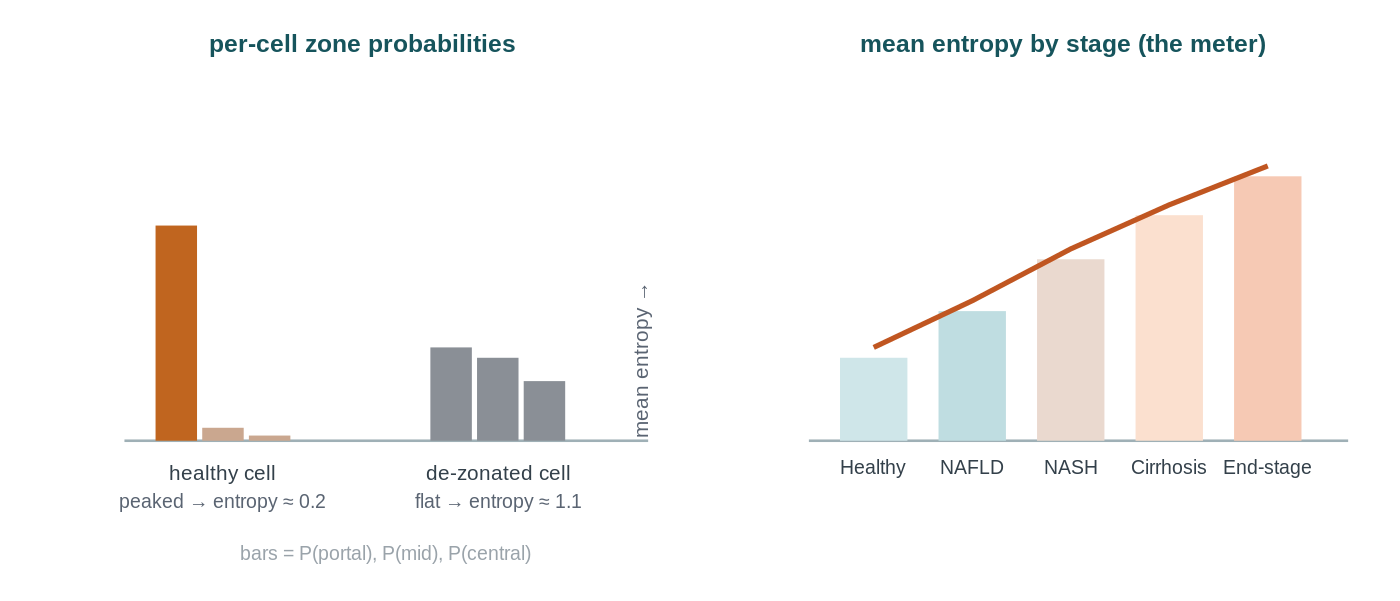
\includegraphics[width=0.85\linewidth]{fig6.png}
\caption{Why the classifier's \emph{confusion} is the signal (illustrative). Left: a healthy hepatocyte
yields a \textbf{peaked} probability vector (the model is sure of its zone $\to$ low entropy); a
de-zonated cell yields a \textbf{flat} one (the model genuinely can't tell $\to$ high entropy). Right:
averaging that entropy per stage gives the headline de-zonation meter --- expected to climb as identity
blurs. Per-zone entropy (not shown) tests whether pericentral confidence falls first (H2).}
\label{fig:entropy}
\end{figure}

\aside{The catch --- and the trick that fixes it (same platform, borrowed labels)}{\textbf{The catch.}
A classifier can ``cheat'' by latching onto \emph{technical} quirks of whatever data it trained on
instead of real biology. Paper~2's main data are \textbf{Visium spots} --- small multi-cell tissue
patches, a different technology. Train on those and ask about Paper~1's \textbf{single nuclei}, and much
of what it ``learned'' would be ``Visium-vs-single-nucleus'' technical difference.
\textbf{The trick.} Paper~2 \emph{also} ran \textbf{snRNA-seq} --- the \emph{same} platform as Paper~1.
So we train on Paper~2's snRNA-seq nuclei and apply to Paper~1's snRNA-seq nuclei: same measurement type
on both sides, so the model can't win by reading the technology --- what carries over is genuine
zonation. \textbf{But where do the labels come from, if Paper~2's snRNA also lost its coordinates?} The
labels do \emph{not} come from the snRNA nuclei's own (lost) positions. Paper~2 profiled the \emph{same
livers two ways} --- spatially (Visium, positions kept) \emph{and} by snRNA-seq. It used the
\textbf{spatial} data to define the porto--central zones, then \textbf{transferred those zone labels
onto its snRNA nuclei} (their repo's \code{parse\_snRNAseq\_combined\_atlas.m}). So training is snRNA
\emph{expression} (same platform as Paper~1) paired with a \emph{zone label borrowed from the spatial
modality}. Our current fallback (until we port that mapping) labels each Paper~2 nucleus by the
signature-tercile rule of \S\ref{sec:scoring}, making the classifier a sanity baseline; swapping in the
spatial-derived labels is the upgrade that makes it ground-truth.}

\textbf{A free sanity check.} Scoring and the classifier are two independent routes to the same answer.
On \emph{healthy} cells, where zonation is intact, they should agree --- and that agreement is built-in
evidence the signal is real biology, not an artefact of either method.

\aside{Entropy is an interpretation, not a direct measurement}{High entropy $\neq$ automatically
de-zonation. A confused prediction means ``the model can't tell which zone'' --- but de-zonation is only
\emph{one} reason. Others: \textbf{too little data in the cell} (a poorly-sequenced nucleus --- a
technical shrug); \textbf{a cell unlike anything trained on} (out-of-distribution, e.g.\ stressed/dying);
\textbf{patient/batch differences}; \textbf{a poorly-calibrated model}; and \textbf{loss of hepatocyte
identity altogether} (not just \emph{zonal} identity). So we call high entropy ``de-zonation'' only when
it is \emph{not} explained by those --- i.e.\ it survives checking against the cell's QC metrics, its
donor/batch, and the module-level diagnostics of \S\ref{sec:rulervalid}. We use a \textbf{calibrated}
classifier (multinomial logistic regression) so the entropy means what we think it does.}

\subsection{Validity: the positive control on healthy liver}
\label{sec:posctrl}

In healthy liver zonation is intact, so the method \emph{must} recover it. When we ran the ruler on
Paper~2's healthy hepatocytes, the coordinate came out as \textbf{one broad hump centred near zero} ---
not two peaks --- and that worried us at first. It shouldn't: a single wide hump is exactly what intact
zonation looks like.

\begin{figure}[h]
\centering
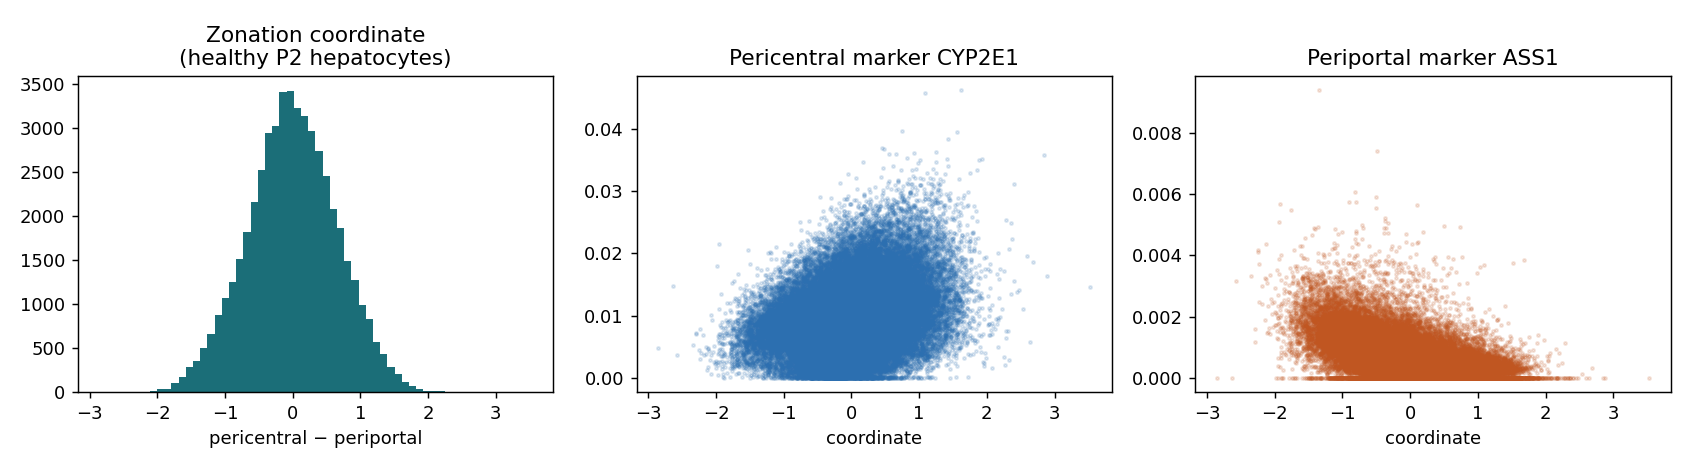
\includegraphics[width=0.95\linewidth]{p2_validation.png}
\caption{The real positive control on healthy liver (Paper~2). The pseudo-zonal coordinate is a single
broad \emph{unimodal} hump (left) --- correct, because zonation is a continuum, not two discrete states.
The proof that the axis is real is the \textbf{marker slopes} (centre, right), not bimodality: the
pericentral marker \gene{CYP2E1} rises with the coordinate and the periportal marker \gene{ASS1} falls.
The ruler works before we ever touch disease data.}
\label{fig:validation}
\end{figure}

\begin{itemize}[leftmargin=1.4em]
\item \textbf{Zonation is a gradient, not a switch.} Cells sit at \emph{every} position from portal to
central, so the coordinate is a continuum; a histogram of a continuum is a single spread-out hump. You
would only see two spikes if hepatocytes came in two discrete states --- which is not the biology. So
unimodal $\neq$ ``no zonation.''
\item \textbf{The proof is in the slopes, not the histogram.} In the same validation figure
\gene{CYP2E1} \emph{rises} with the coordinate and \gene{ASS1} \emph{falls}. That monotonic ordering is
the evidence the axis is real zonation; with no zonation those scatters would be flat clouds.
\item \textbf{De-zonation is therefore a change in \emph{shape}, not in \emph{modality}.} We never
expect ``two peaks become one.'' We expect the one hump to get \textbf{narrower} across disease
(variance shrinks toward the middle) and the \gene{CYP2E1}/\gene{ASS1} slopes to \textbf{flatten}. So
the healthy single-peak-with-correct-slopes result is a \emph{pass}, not a problem.
\end{itemize}

This positive control (Step~5) is paired with the ruler-validity diagnostics (Step~5b,
\S\ref{sec:rulervalid}), which decide --- before any disease claim --- \emph{whether and how} the ruler
itself holds up as disease advances.

\subsection{De-zonation is a population property}
\label{sec:popprop}

We define de-zonation \textbf{operationally}, as the degradation of three properties of the cell
\emph{population} --- not of any single cell's coordinate, which we never treat as a true position.

\begin{enumerate}[leftmargin=1.6em]
\item \textbf{Mutual exclusivity.} In healthy liver a hepatocyte is high-pericentral \emph{or}
high-periportal, so the two scores are strongly \emph{anti}-correlated across cells. De-zonation $=$
cells expressing \emph{both} at once $\to$ that anti-correlation weakens.
\item \textbf{Spread.} Healthy hepatocytes span the whole axis, so the coordinate is a \emph{wide}
distribution (typically a single broad hump --- a continuum, not two peaks); collapse bunches cells
toward the middle (narrow). We track variance/IQR --- the \emph{width} is the signal, regardless of the
hump's exact shape (Fig.~\ref{fig:ridgeline}).
\item \textbf{Internal coherence.} Do the pericentral genes still co-vary \emph{with each other} --- is
the program still a coherent module? (Step~5b.)
\end{enumerate}

\textbf{Why this isn't circular:} assigning each cell a coordinate from its expression does \emph{not}
predetermine any of (1)--(3) --- a disease that preserved zonation would keep strong anti-correlation
and wide spread, both fully allowed outcomes. The 1-D coordinate alone is ambiguous (a middle value $=$
``expresses neither'' \emph{or} ``expresses both''), which is exactly why the honest metrics are these
structural ones.

\aside{The donor is the unit (a preview of \S\ref{sec:stats})}{Every population metric above is computed
\emph{per donor} ($\approx$47 of them), never on the pooled $\sim$69{,}426 cells. Cells from one donor
share that donor's genetics, batch and biology, so treating them as independent inflates the sample size
from $\approx$47 to $\sim$10$^5$ and produces an absurdly tiny, meaningless p-value --- the error called
\textbf{pseudoreplication}. The fix is a two-step pattern used throughout: collapse cells to one number
per donor, then run the donor-level test.}

\subsection{Comparing stages without fooling ourselves (the statistics)}
\label{sec:stats}

Every test below shares one governing rule, so we state it once and apply it everywhere.

\aside{The one rule: the donor is the unit of inference}{We have $\approx$47 donors. Each contributes
thousands of cells, from which we compute \emph{one} summary per donor. The biological question is a
statement about \textbf{donors}, so the sample size that matters is $n\approx 47$, \emph{not} $\sim$69k
cells. Run a test on cell-level values and you silently inflate $n$ from 47 to $\sim$10$^5$; the p-value
becomes absurdly tiny and meaningless (\textbf{pseudoreplication}). The fix is two-step: (1)~collapse
cells to one number per donor; (2)~run the donor-level test. When we resample for confidence intervals,
we resample \emph{donors}, not cells. DE achieves this by \emph{pseudobulk}: aggregating to
donor$\times$zone before testing.}

\paragraph{H1 --- the ordered-trend tests.} The stages are \emph{ordered}, and ordering is information:
a test that uses it is more powerful than one that ignores it.

\emph{Spearman's $\rho$} is Pearson's correlation computed on the \emph{ranks} of stage and score, so
it detects any monotone relationship regardless of exact spacing or outliers. With no ties it reduces
to the shortcut
\begin{equation}
\rho \;=\; 1 - \frac{6\sum_i d_i^2}{n\,(n^2-1)},
\end{equation}
where $d_i$ is the difference between donor $i$'s two ranks and $n$ is the number of donors ($\rho=+1$
perfectly increasing, $0$ no trend; with the heavily-tied stages use the general Pearson-on-mid-ranks
form, as \code{scipy.stats.spearmanr} does).

\emph{Jonckheere--Terpstra (JT)} is the purpose-built ordered cousin of Kruskal--Wallis. Its null is
``all $k$ stage distributions identical''; its alternative the directional ``medians don't decrease as
you walk along the stages,'' $M_1\le M_2\le\cdots\le M_k$. It builds its statistic from the
Mann--Whitney counts of every ordered stage-pair, $J=\sum_{a<b}U_{ab}$ with
$U_{ab}=\#\{x_b>x_a\}$, and spends all its power on the one pattern we predicted in advance --- a march
in stage order --- so when that ordering is real it detects it with a smaller sample (the cost: a
non-monotone, up-then-down effect can slip past it). Under $H_0$, $J$ has a known mean and variance,
giving a one-sided normal $z=(J-\mu_J)/\sigma_J$; for small/tied samples we prefer a permutation null.

\emph{Donor-level bootstrap CI.} A p-value says ``is the trend distinguishable from zero?''; a
confidence interval says ``how big, and how sure.'' We resample the $\approx$47 \textbf{donors} with
replacement $B\approx2000$--$10000$ times, recompute $\rho$ each time, and take the 2.5/97.5 percentiles.
Resample \emph{donors}, not cells --- the resampling unit must match the inference unit, or the CI is
far too narrow (pseudoreplication again). If the 95\% CI excludes 0 the trend is significant in the
bootstrap sense, and the width reports precision honestly.

\emph{Permutation negative control.} Keep the scores, randomly reassign stage labels across donors,
recompute $\rho$ thousands of times to build the empirical null. The two-sided p-value (with the
standard $+1$) is $p=(\#\{|\rho^\ast|\ge|\rho|\}+1)/(B+1)$. Run on shuffled labels the observed
statistic should land in the bulk of the null ($p\approx0.5$) --- a pipeline that ``finds'' a trend in
shuffled data is broken.

\paragraph{H3 --- association, with the stage confound removed.} The trap: \emph{both} de-zonation and
plasticity tend to rise with stage, so a naive pooled correlation across all cells looks positive even
if the two are unrelated within any single donor --- a textbook Simpson's-paradox confound. The whole
job is to remove it, never to pool.

\emph{Within-donor correlation, then aggregate.} Compute the correlation \textbf{inside each donor}
(where stage is held fixed and cannot drive a spurious link), then aggregate the $\approx$47
within-donor $\rho_d$ values and test whether their centre sits above zero (sign test / Wilcoxon
signed-rank), reporting both the mean $\rho$ (strength) and the fraction of donors with $\rho_d>0$
(consistency).

\emph{OLS with covariates.} The regression equivalent is
\begin{equation}
\text{plast} \;\sim\; \text{dez} + C(\text{stage}) + C(\text{donor}),
\end{equation}
where $C(\cdot)$ are categorical dummy terms that soak up each stage's and each donor's baseline
plasticity; the coefficient $\beta$ on \code{dez} is the partial association after stage and donor are
removed. Including $C(\text{donor})$ makes each comparison \emph{within} a donor --- the regression
analogue of the within-donor correlation. Use clustered standard errors or a donor random effect, or the
\code{dez} p-value is over-confident (pseudoreplication in regression clothing).

\emph{Mann--Whitney U.} Where we contrast two groups directly (de-zonated vs zonated), pool and rank all
values and ask whether one group hogs the high ranks. From the rank-sum $R_1$ of group~1,
\begin{equation}
U_1 = R_1 - \frac{n_1(n_1+1)}{2},\qquad U_1+U_2=n_1 n_2,\qquad \mathrm{AUC}=\frac{U_1}{n_1 n_2}.
\end{equation}
Its effect size is the rank-biserial $r = 2\cdot\mathrm{AUC}-1$, always reported beside the p-value.

\paragraph{H2 --- differential expression with FDR.} Once every hepatocyte has a coordinate, we bin
cells into pseudo-zones and ask, within a zone, which genes change across disease stage. The danger is
volume: testing $\sim$20{,}000 genes at $p<0.05$ yields $\sim$1{,}000 false positives from noise alone
(the ``throw enough nets and you catch plastic bottles'' problem of Lecture~5). The
\textbf{Benjamini--Hochberg (BH)} procedure controls the \emph{false discovery rate} --- the expected
fraction of false positives \emph{among the genes we call significant} --- rather than forbidding any
false positive at all (which Bonferroni's $\alpha/m$ does, losing nearly all real signal at this scale).
Sort the $m$ p-values $p_{(1)}\le\cdots\le p_{(m)}$, find the largest rank $k$ with
\begin{equation}
p_{(k)} \;\le\; \frac{k}{m}\,q \qquad (e.g.\ q=0.05),
\end{equation}
and declare ranks $1\ldots k$ significant; the \textbf{q-value} of a gene is the smallest FDR at which
it would be called. Everything we report as ``significant'' is at $q<0.05$, never a raw p-value --- and
always paired with an \textbf{effect size} (log fold-change, or the coordinate$\times$stage slope of
Step~7), because a tiny $q$ says a change is \emph{real}, not that it is \emph{large}.

To respect the donor as the unit we run DE as \textbf{pseudobulk}: aggregate expression per
donor$\times$zone, then fit per gene the interaction model
\begin{equation}
\text{expr} \;\sim\; \text{coord} + \text{stage} + \text{coord}{:}\text{stage},
\end{equation}
in which the \emph{interaction term} (``this gene's zonal slope weakens with stage'') is the honest
``lost zonal pattern'' test. \textbf{Avoiding circularity:} because the coordinate is built from the
signature genes, the driver test must not simply re-test them. We use a \textbf{random held-out gene
split} --- define the coordinate on one half of the zonation genes, test collapse on the other ---
\textbf{repeated $K\approx20$--$50$ times}, reporting the \emph{distribution} of the result across
splits (a robust signal holds across most splits; this is meaningful only with the full
$\sim$1{,}640-gene set, not 20 landmarks), and we exclude/flag signature genes from any ``driver'' claim.

\noindent\textbf{In code.} \code{src/steps/step7\_de.py} --- pseudobulk (donor$\times$zone), per-gene
\code{expr $\sim$ coord + stage + coord:stage}, \code{multipletests(method='fdr\_bh')}.

\aside{The whole logic in one line}{table $\to$ clean it (QC, normalize) $\to$ trust no single gene
(dropout) $\to$ pool genes into a coordinate (signature, both ways) $\to$ sharpen with a same-platform
classifier (entropy $=$ blur) $\to$ check the ruler still holds (5b) $\to$ compare stages with
donor-level, FDR-controlled tests.}

\subsection{When does the ruler stop being a ruler? (validity controls, Step~5b)}
\label{sec:rulervalid}

Here is the project's deepest risk. The ruler is calibrated on healthy tissue, but disease may corrupt
the very genes it relies on. A coordinate collapsing to the middle could mean (a)~genuine de-zonation,
(b)~the marker genes globally crashing for unrelated reasons (the tick-marks fall off the ruler), or
(c)~the signature dissolving into noise. The raw number can't tell these apart --- so we measure the
\emph{structure} of the signature per stage:
\begin{enumerate}[leftmargin=1.6em]
\item \textbf{Internal coherence} --- mean pairwise correlation among pericentral genes (and among
periportal): is the ruler still a coherent module?
\item \textbf{Cross-program anti-correlation} --- correlation between the two module scores across
cells: true de-zonation, and robust to global shifts.
\item \textbf{Split-half reproducibility} --- correlate two coordinates from random half-signatures.
\item \textbf{Program-off vs restriction-lost} --- track each module's mean magnitude alongside the
co-expression rate, distinguishing a module switched \emph{off} (program lost) from one still on but
co-expressed with its opposite (positional restriction lost).
\end{enumerate}
These diagnostics let us say which kind of breakdown we are seeing rather than assuming the convenient
one.

\clearpage
% ====================================================================
\section{Work plan}
\label{sec:workplan}
% ====================================================================

The slow plumbing is done (\S\ref{sec:prework}); the hackathon is the science. Every step below already
has a \textbf{stub file} (signature $+$ docstring with algorithm, I/O and acceptance check) and a
\textbf{plotting function}; the donor-level reference implementation for the statistical steps lives in
\code{src/pipeline.py}, driven by \code{src/run\_all.py} with settings in \code{src/config.py} and
plots in \code{src/plotting/artefacts.py}.

\subsection{Inputs and environment}

Raw inputs live in \code{data/raw/}; the two big ones were already converted once into Python-native
files in \code{data/processed/}. The pipeline reads only the processed files --- it never touches the
\code{.rds} or \code{.mat} again. Paper~1 ($\sim$2.6\,GB Seurat \code{.rds}) $\to$ \code{counts.mtx} $+$
metadata via an R export (\code{src/prep/01\_extract\_paper1\_hepatocytes.R}), read with
\code{scipy.io.mmread}. Paper~2 ($\sim$2.0\,GB MATLAB v7.3 \code{.mat} $=$ HDF5) $\to$
\code{paper2\_train.npz} via \code{h5py} (\code{src/prep/02\_convert\_paper2\_mat.py}). After these two
one-off prep steps the analysis is pure Python: \code{scanpy/anndata} (or \code{scipy.sparse}) for
single-cell handling; \code{numpy/scipy/pandas/scikit-learn} for normalization, the signature, the
classifier and statistics; \code{statsmodels} for \code{multipletests(method='fdr\_bh')};
\code{matplotlib/seaborn} for figures. Where the course expects understanding (normalization, FDR, the
classifier) we implement it explicitly rather than hide behind a one-liner.

\subsection{The live hackathon steps (1--9)}

\begin{table}[h]
\centering\small
\caption{The nine steps, their code stubs, and the hypothesis each answers.}
\label{tab:steps}
\begin{tabular}{@{}p{0.13\linewidth} p{0.38\linewidth} p{0.40\linewidth}@{}}
\toprule
\textbf{Step} & \textbf{Code stub} & \textbf{Artefact / answers}\\
\midrule
1 Ruler & \code{prep/02\_convert\_paper2\_mat.py}; \code{signatures/} & A1 signatures (full $+$ landmark)
$+$ zone-labelled training set\\
2 Load/QC & \code{steps/step2\_load\_qc.py} & A2 clean normalized hepatocyte matrix ($\sim$69k) $+$
counts\\
3 Harmonize & \code{steps/step3\_harmonize.py} & A3 gene map (symbol/Ensembl, report mapping rate)\\
4 Score & \code{steps/step4\_score.py} & A4 per-cell coordinate (both gene sets)\\
4b Classifier & \code{steps/step4b\_classifier.py} & A4 zone-probability vector $+$ entropy\\
5 Validate & \code{steps/step5\_validate.py} & A5 healthy positive control (Fig.~\ref{fig:validation})\\
5b Ruler diag. & \code{steps/step5b\_ruler\_diagnostics.py} & A5b validity (coherence / anti-corr /
split-half / decomposition)\\
6 Collapse & \code{steps/step6\_collapse.py} & A6 collapse curve $\cdot$ \textbf{H1}\\
7 Zone DE & \code{steps/step7\_de.py} & A7 pseudobulk DE $+$ FDR $\cdot$ \textbf{H2}\\
8 Plasticity & \code{steps/step8\_plasticity.py} & A8 de-zonation$\leftrightarrow$plasticity $\cdot$
\textbf{H3}\\
9 Bonus & \code{steps/step9\_bonus\_enrichment.py} & A9 hypergeometric enrichment (Paper~3)\\
\bottomrule
\end{tabular}
\end{table}

\textbf{Steps 1--3 (reference, load, harmonize).} Build the ruler from Paper~2 --- transcriptome-wide
set ($q<0.05$, well-expressed, present in Paper~1, sided by Center-of-Mass; the default) plus the exact
landmark set verbatim; \emph{reserve a random held-out subset} (e.g.\ 30\%) of the zonation genes that
builds neither the coordinate nor the classifier, for the non-circular collapse test in Step~7; port
\code{parse\_snRNAseq\_combined\_atlas.m} to attach a spatial-derived zone label to each Paper~2 nucleus.
Load Paper~1 hepatocytes, inherit the authors' QC (sanity check \gene{ALB}-positive cells; optional
lowest-UMI sensitivity filter), re-normalize from \code{counts} (\S5.2), and build a per-stage/per-donor
count table (donor IDs feed the bootstrap). Reconcile gene identifiers, intersect signatures to the
shared gene set (report surviving sizes), and use z-scored/rank-based features so the score measures
portal-vs-central, not snRNA-vs-Visium.

\textbf{Steps 4--5b (place \& validate).} Compute \code{zonation\_coord} with both gene sets and confirm
agreement; train the calibrated classifier on Paper~2's zone-labelled nuclei, evaluate by held-out
confusion matrix \emph{on Paper~2 first}, then apply to Paper~1 (record predicted zone, probability
vector, entropy). Validate on Paper~1's healthy donors (Step~5): markers track the coordinate
(\gene{GLUL}/\gene{CYP2E1} up, \gene{ASS1}/\gene{HAL} down, quantified by Spearman), classifier
confident (low entropy); the proof is the marker slopes, not bimodality (\S\ref{sec:posctrl}).
\textbf{If healthy cells do not separate, stop and fix scoring before touching disease data.} Run the
four ruler-validity diagnostics across all stages (Step~5b, \S\ref{sec:rulervalid}).

\textbf{Step 6 (collapse, H1).} Compute each metric \emph{per donor} --- classifier prediction-entropy
(headline), coordinate spread, axis separability, marker anti-correlation --- then test the ordered
trend on the $\approx$47 per-donor values (Jonckheere--Terpstra / Spearman), with a donor-level
bootstrap CI and a stage-label-shuffle negative control. The pseudo-code makes the
\emph{donor-is-the-unit} discipline explicit:
\begin{verbatim}
for d in donors:                      # UNIT = DONOR (~47), never cell
    spread[d]   = std(coord[donor==d])
    anticorr[d] = spearman(pc[donor==d], pp[donor==d])
    entropy[d]  = mean(cell_entropy[donor==d])
rank   = stage_rank[donor_stage]                   # Healthy=0 ... End-stage=4
rho,p  = spearman(rank, spread)                    # ordered trend on ~47 values
CI     = bootstrap_over_DONORS(rho, B=2000)        # error bars
p_perm = shuffle_stage_labels(rho, B=2000)         # negative control
PASS if spread DOWN, anticorr -> 0, CI excludes 0, p_perm small
\end{verbatim}

\begin{figure}[h]
\centering
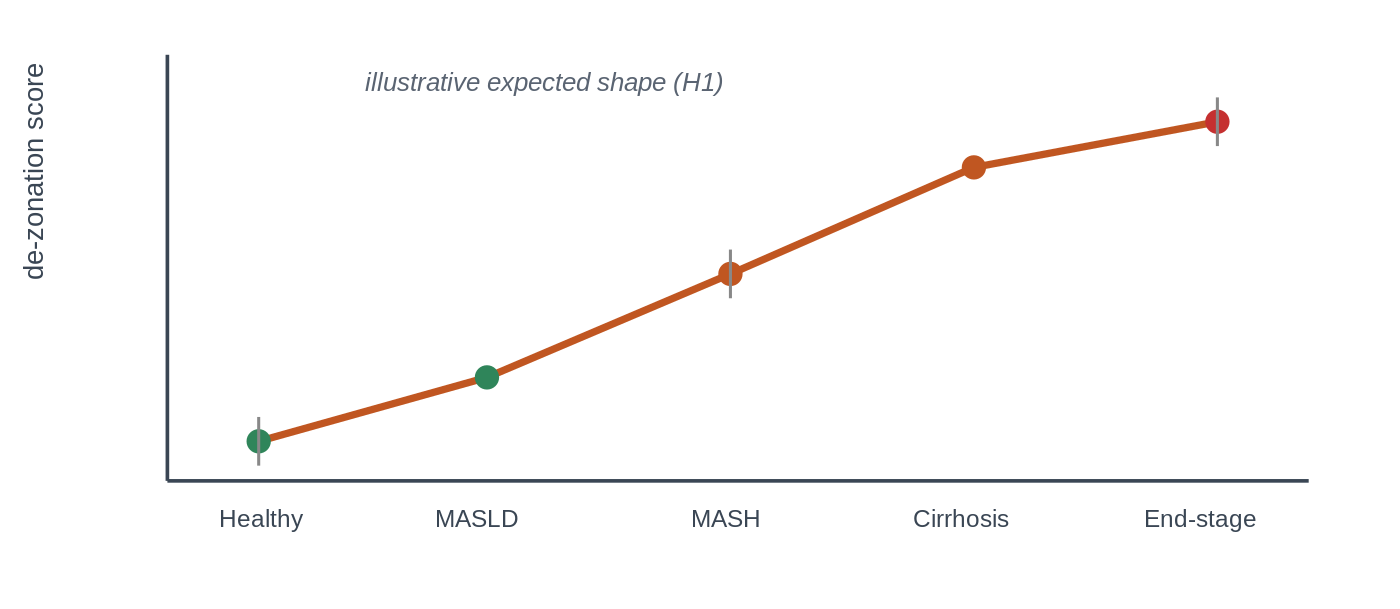
\includegraphics[width=0.7\linewidth]{fig8.png}
\caption{The headline deliverable (mock-up): a de-zonation metric rising monotonically across stages
with donor-bootstrap confidence intervals --- one value per donor, tested across the ordered stages
(Step~6). Shape illustrative; the real curve is the result.}
\label{fig:collapse}
\end{figure}

\textbf{Step 7 (zone DE, H2).} Bin hepatocytes into pseudo-zones (portal/mid/central terciles), then
pseudobulk per donor$\times$zone and test the stage effect, BH-FDR across genes. Guards against
circularity: exclude signature/classifier genes from driver claims; use the $K\approx20$--$50$ repeated
held-out gene splits; and prefer the per-gene \code{expr $\sim$ coord + stage + coord:stage} interaction
term as the honest ``lost zonal pattern'' test.
\begin{verbatim}
zone = tercile(coord)                              # portal / mid / central
for z in [portal, central]:
    PB = pseudobulk(expr, by=(donor, zone))        # donor x gene mean log1p-CP10k
    for g in genes_detected_in(z):                 # >=10% of zone's cells
        fit:  PB[g] ~ coord + stage + coord:stage  # OLS on the donor aggregates
        p[g] = pvalue(coord:stage)                 # does the ZONAL SLOPE change?
    q = BH(p)
report q<0.05 EXCLUDING signature genes            # circularity guard
\end{verbatim}

\textbf{Step 8 (plasticity link, H3).} Score each hepatocyte for a cholangiocyte/plasticity signature
(a \emph{separate} axis, \S\ref{sec:twobreaks}), then test the link within donor/within stage --- per-
donor correlations aggregated, or \code{plast $\sim$ dez + C(stage) + C(donor)} --- never pooled, where
late disease would trivially show more of both and fake a correlation. Report effect size beside p.

\subsection{Work division, risk register, and success criteria}

The detailed timeline and two-person split appear in \S\ref{sec:timeline}. Key risks and mitigations:
platform batch dominating placement (rank/z-scored features; train on Paper~2's own snRNA-seq; validate
on Paper~1 healthy cells); the ruler dissolving in disease (Step~5b decides interpretation before any
claim); pseudoreplication (donor-level inference throughout; donor bootstrap and donor-label-shuffle
control); out-of-distribution disease nuclei (flag low-confidence cells; cross-check entropy against QC
and the signature score); gene-set circularity (exclude signature genes from driver claims; K-repeated
held-out splits; interaction-term test); and the known GSM metadata swap (use the corrected GEO version;
print donor counts per stage at load time). \textbf{Statistical-rigor checklist:} significance always at
BH-FDR $q<0.05$, never raw p; stage effect via an \emph{ordered} trend test; donor-level resampling;
DE as pseudobulk (donor$\times$zone) with the H2 collapse tested via the coordinate$\times$stage
interaction on K-repeated held-out gene splits; coordinate computed both transcriptome-wide and on the
landmark set, shown to agree; a positive control (Step~5) and a negative control (shuffled labels);
classifier judged by held-out accuracy on Paper~2 before use on Paper~1; effect sizes beside p/q.

\clearpage
% ====================================================================
\section{Limitations \& honest scope}
% ====================================================================

\begin{figure}[h]
\centering
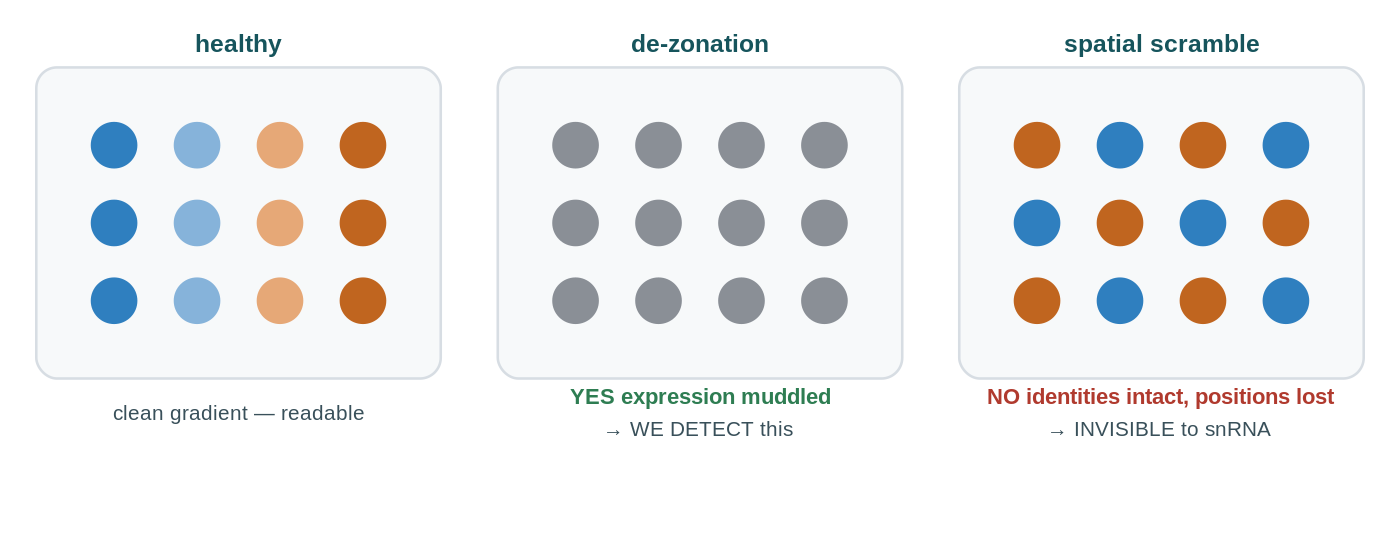
\includegraphics[width=0.85\linewidth]{fig7.png}
\caption{What the method can and cannot see. Each dot is a cell, coloured by expressed identity (blue
$=$ periportal, orange $=$ pericentral, grey $=$ both/neither). We detect de-zonation when the
\textbf{expression program} degrades (middle: cells stop committing) --- that is real and measurable. We
are \textbf{blind} to pure spatial scrambling (right): if cells kept distinct identities but were
physically rearranged, a dissociated method records no change, because the positions were never measured.
This honest scope limit is why a future spatial-disease study would complement, not duplicate, our
result.}
\label{fig:scope}
\end{figure}

\begin{itemize}[leftmargin=1.4em]
\item \textbf{Blind to pure spatial scrambling.} We measure loss of the \emph{expression} program, not
physical re-arrangement. If diseased cells kept their gene-identity but were shuffled in space (a
periportal-type cell sitting where pericentral cells belong), our method --- like any dissociated
snRNA method --- would report \emph{no} change, because the positions were never recorded. Detecting
architectural scrambling with intact expression needs spatial data on the \emph{diseased} tissue ---
the very thing that does not yet exist.
\item \textbf{Pseudo-zonal, not $(x,y)$.} The ruler is a 1-D axis, so we recover a reconstructed
zonation coordinate, never a physical location. We never claim ``predicted spatial position.''
\item \textbf{Ruler-validity.} The ruler is calibrated on healthy tissue and may degrade in disease;
Step~5b (\S\ref{sec:rulervalid}) is exactly the honesty check that says \emph{whether} and \emph{how}
the ruler holds at each stage, so the collapse is interpreted correctly rather than conveniently.
\item \textbf{Associational, not causal.} H1--H3 establish that zonation erodes with stage, which
programs erode first, and that de-zonation tracks plasticity --- not that one \emph{causes} another. The
optional Paper~3 bonus (next section) is likewise an enrichment association, not a causal claim.
\end{itemize}

% ====================================================================
\section{Optional bonus: does the collapse track inherited MASLD risk? (Paper~3)}
% ====================================================================

\textbf{The question, sharpened.} Paper~3 (Zhu \emph{et~al.}, \emph{Nat.\ Genet.} 2026) maps MASLD
\textbf{inherited risk variants} to the genes they regulate (snATAC-seq $+$ a massively-parallel
reporter assay $\to$ a list of \emph{risk-variant target genes}). We ask one precise thing: are the
genes whose zonal pattern collapses earliest (our Step-7 hits) over-represented among those
inherited-risk target genes --- more than chance? A ``yes'' means the cell-state breakdown we measure
and germline susceptibility converge on the same molecular targets; a ``no'' means de-zonation is mostly
an \emph{acquired}, downstream process. Either answer is publishable-grade context, and neither is needed
for H1--H3.

\textbf{The exact test --- a hypergeometric gene-set overlap test} (light, no new heavy data). Let the
\emph{background} be the genes \emph{actually testable} in Step~7 (detected in the zone, survived
pseudobulk) --- \emph{not} all $\sim$20k genes. With $N=|\text{background}|$, $K=|\text{background}\cap
\text{risk}|$ successes in the population, a draw of size $n=|\text{hits}|$ of which $k=|\text{hits}\cap
\text{risk}|$ are successes, the one-sided enrichment p-value is
\begin{equation}
p \;=\; \sum_{i=k}^{\min(n,K)} \frac{\binom{K}{i}\binom{N-K}{\,n-i\,}}{\binom{N}{n}}
\;=\; \texttt{hypergeom.sf}(k-1,\,N,\,K,\,n),
\qquad
\text{fold} = \frac{k/n}{K/N}\ (>1 \Rightarrow \text{enrichment}).
\end{equation}

\aside{Why the background matters (the easy way to fool yourself)}{Testing against all 20{,}000 genes
guarantees fake enrichment, because both lists are biased toward highly-expressed liver genes. The
honest background is the set of genes that \emph{could} have been called in Step~7 (detected $+$ tested),
ideally expression-matched to the hit list. \textbf{Interpretation:} fold $>1$ with BH $q<0.05$ $\to$
genetics$\times$cell-state convergence; fold $\approx1$ $\to$ independent processes. \textbf{Caveats:}
variant$\to$gene mapping is imperfect; small hit lists give wide CIs; the result is associational, not
causal. \textbf{Code:} \code{src/steps/step9\_bonus\_enrichment.py} ($\sim$30~min, gene-list only). It is
genuinely additive, cheap (one hypergeometric test you already know from Lecture~5), and strictly
optional --- the project stands fully on H1--H3 without it, so it can never sink the timeline.}

\clearpage
% ====================================================================
\section{Timeline \& work division}
\label{sec:timeline}
% ====================================================================

\begin{table}[h]
\centering\small
\caption{Timeline. Step~5 (the positive control) must pass early --- it is the critical path.}
\label{tab:timeline}
\begin{tabular}{@{}p{0.10\linewidth} p{0.46\linewidth} p{0.40\linewidth}@{}}
\toprule
\textbf{When} & \textbf{Goal} & \textbf{Done when\ldots}\\
\midrule
Prep & Data downloaded $+$ converted; signatures (A1) $+$ QC'd hepatocytes (A2) ready & Both datasets
load in one notebook\\
Day~1 & Harmonize (A3), place all cells (A4), validate (A5, A5b) & Method recovers zonation in healthy
donors; score \& classifier agree\\
Day~2 & Collapse curve (A6), DE (A7), plasticity (A8), write-up (A9) & H1--H3 answered with controlled
statistics\\
\bottomrule
\end{tabular}
\end{table}

\aside{Critical path \& minimum viable result}{If the coordinate recovers healthy zonation by end of
Day~1, the rest is mechanical --- do not start the collapse analysis until the positive control passes.
The project still fully succeeds on a reduced scope: the signature coordinate (Step~4a, no classifier)
$+$ the healthy positive control (Step~5) $+$ the donor-level collapse trend for H1 (Step~6) is a
complete, defensible story on its own. Everything beyond --- the classifier/entropy reader, the
pseudobulk DE for H2, the plasticity link for H3, and the Paper~3 bonus --- is layered on in that order,
each independently droppable. Build H1 end-to-end first, then add upward.}

\textbf{Work division.} \textbf{Roee} owns the harder statistics/methods spine: parsing Paper~2 and
building the signatures and classifier training set (Step~1), the harmonization/batch strategy (Step~3),
the validation and ruler diagnostics (Steps~5, 5b), and the donor-level collapse statistics and
plasticity link (Steps~6, 8) plus figures. \textbf{Shira} owns the disease-data wrangling, baseline,
validation support and figures: downloading and QC-ing the Paper~1 hepatocytes (Step~2), the scoring and
classifier scaffold and placing all cells (Step~4), the zone-binned pseudobulk DE with FDR (Step~7), and
the write-up, reproducibility and stretch bonus.

\begin{table}[h]
\centering\small
\caption{Two-person split across the phases.}
\label{tab:split}
\begin{tabular}{@{}p{0.14\linewidth} p{0.42\linewidth} p{0.42\linewidth}@{}}
\toprule
\textbf{Phase} & \textbf{Roee --- stats/methods spine} & \textbf{Shira --- disease data \& baseline}\\
\midrule
Prep & Parse Paper~2; signatures (full $+$ landmark) $+$ training set (Step~1) & Download $+$ QC Paper~1
hepatocytes (Step~2)\\
Day~1 AM & Harmonize, batch strategy (Step~3) & Scoring $+$ classifier scaffold (Step~4)\\
Day~1 PM & Validation $+$ ruler diagnostics (5, 5b) & Place all cells (Step~4 finished)\\
Day~2 AM & Collapse metrics $+$ trend stats (Step~6) & Zone-binned DE $+$ FDR (Step~7)\\
Day~2 PM & Plasticity link (Step~8) $+$ figures & Write-up, reproducibility, stretch\\
\bottomrule
\end{tabular}
\end{table}

\clearpage
% ====================================================================
\section{Glossary}
% ====================================================================

\begin{table}[h]
\centering\small
\begin{tabular}{@{}p{0.30\linewidth} p{0.66\linewidth}@{}}
\toprule
\textbf{Term} & \textbf{Meaning}\\
\midrule
Hepatocyte / Cholangiocyte & Main metabolic liver cell / bile-duct cell (hepatocytes can drift toward
this identity in disease)\\
Lobule & Hexagonal liver unit (0.5--1\,mm)\\
Porto--central axis & Blood-flow gradient from portal inlet to central vein\\
Zonation / De-zonation & Position-dependent division of labour / its loss in disease (a population
property, not one cell's coordinate)\\
Plasticity & Loss of cell-type identity (hepatocyte$\to$cholangiocyte); a separate axis from zonation\\
Periportal / Pericentral & Relatively oxygen-rich (portal) / oxygen-poor (central) ends of the axis\\
MASLD / MASH & Fatty liver disease / steatohepatitis (fat $+$ inflammation); older labels NAFLD/NASH\\
snRNA-seq & Single-nucleus RNA-seq; survives hard tissue, loses spatial coordinates, intron-heavy\\
Spatial transcriptomics & Expression measured with position kept (Visium / Visium HD / MERFISH /
PhenoCycler)\\
UMI / Dropout & Counted unique molecule / a technical zero (gene on but missed)\\
QC & Quality control: discarding junk/low-quality cells before analysis\\
Signature score & Pooled (background-subtracted) expression of a gene set (robust to single-gene
dropout)\\
Landmark / Transcriptome-wide & Paper~2's anchor genes (baseline) / the full $\sim$1{,}640 zonated genes
(default); coordinate computed both ways\\
Zone classifier / entropy & Model predicting a cell's zone; flat (high-entropy) prediction $=$
de-zonated\\
Zonation coordinate & Reconstructed 1D portal$\leftrightarrow$central position (pseudo-spatial, not
$x,y$)\\
DE / FDR (Benjamini--Hochberg) & Testing which genes change / controlling false positives across many
tests (q-value)\\
Pseudobulk & Aggregating a donor's cells (per zone) to one profile before testing --- the donor-level
fix for DE\\
Pseudoreplication & Wrongly treating many cells from few donors as independent\\
\bottomrule
\end{tabular}
\end{table}

% ====================================================================
\section{References}
% ====================================================================

\begin{enumerate}[leftmargin=1.6em]
\item \textbf{Paper~1.} Gribben C, Galanakis V, Calderwood A, et~al. \emph{Acquisition of epithelial
plasticity in human chronic liver disease.} Nature (2024). doi:10.1038/s41586-024-07465-2. Data: GEO
GSE202379 (\code{GSE202379\_SeuratObject\_AllCells.rds.gz}); code
github.com/Core-Bioinformatics/MASLD-NASH.
\item \textbf{Paper~2.} Yakubovsky O, Bahar Halpern K, Shir S, et~al. \emph{A spatial atlas of the
healthy human liver from live donors.} Nature (2026). doi:10.1038/s41586-026-10377-y. Data: Zenodo
17735506 / 17735558 / 17735587 (the latter holds \code{zon\_struct\_all\_full.mat} and
\code{combined\_scRNAseq\_atlas\_M5M6M7M8.mat}); code github.com/OranYak/Human-liver; web app
shalevapps.weizmann.ac.il/liver\_app.
\item \textbf{Paper~3.} Zhu B, et~al. \emph{Integrative analyses \ldots\ risk alleles for metabolic
liver disease.} Nature Genetics (2026). doi:10.1038/s41588-026-02617-8.
\item \textbf{Paper~4.} Martin OP, et~al. \emph{Single-cell atlas of human liver and blood immune cells
across fatty liver disease stages.} Nature Immunology (2025). doi:10.1038/s41590-025-02255-y.
\item Benjamini Y, Hochberg Y. \emph{Controlling the false discovery rate.} J.\ R.\ Statist.\ Soc.\ B
(1995).
\item Halpern KB, Itzkovitz S, et~al. \emph{Single-cell spatial reconstruction reveals global division
of labour in the mammalian liver.} Nature (2017) --- the zonation-reconstruction concept.
\item Course materials, Computational Genomics 76553: Ex~1 (alignment), Ex~2 (library complexity),
Lec~5 (multiple testing / FDR), Lec~15--16 (single-cell clustering).
\end{enumerate}

\bigskip
\noindent\textit{\small Planning $+$ study aid for the hackathon. Paper figures/tables are pointed to,
not reproduced; verify exact supplementary file names and accession contents at download time.}

\end{document}
